\documentclass[twoside]{book}

% Packages required by doxygen
\usepackage{fixltx2e}
\usepackage{calc}
\usepackage{doxygen}
\usepackage[export]{adjustbox} % also loads graphicx
\usepackage{graphicx}
\usepackage[utf8]{inputenc}
\usepackage{makeidx}
\usepackage{multicol}
\usepackage{multirow}
\PassOptionsToPackage{warn}{textcomp}
\usepackage{textcomp}
\usepackage[nointegrals]{wasysym}
\usepackage[table]{xcolor}

% NLS support packages
\usepackage[spanish]{babel}
% Font selection
\usepackage[T1]{fontenc}
\usepackage[scaled=.90]{helvet}
\usepackage{courier}
\usepackage{amssymb}
\usepackage{sectsty}
\renewcommand{\familydefault}{\sfdefault}
\allsectionsfont{%
  \fontseries{bc}\selectfont%
  \color{darkgray}%
}
\renewcommand{\DoxyLabelFont}{%
  \fontseries{bc}\selectfont%
  \color{darkgray}%
}
\newcommand{\+}{\discretionary{\mbox{\scriptsize$\hookleftarrow$}}{}{}}

% Page & text layout
\usepackage{geometry}
\geometry{%
  a4paper,%
  top=2.5cm,%
  bottom=2.5cm,%
  left=2.5cm,%
  right=2.5cm%
}
\tolerance=750
\hfuzz=15pt
\hbadness=750
\setlength{\emergencystretch}{15pt}
\setlength{\parindent}{0cm}
\setlength{\parskip}{3ex plus 2ex minus 2ex}
\makeatletter
\renewcommand{\paragraph}{%
  \@startsection{paragraph}{4}{0ex}{-1.0ex}{1.0ex}{%
    \normalfont\normalsize\bfseries\SS@parafont%
  }%
}
\renewcommand{\subparagraph}{%
  \@startsection{subparagraph}{5}{0ex}{-1.0ex}{1.0ex}{%
    \normalfont\normalsize\bfseries\SS@subparafont%
  }%
}
\makeatother

% Headers & footers
\usepackage{fancyhdr}
\pagestyle{fancyplain}
\fancyhead[LE]{\fancyplain{}{\bfseries\thepage}}
\fancyhead[CE]{\fancyplain{}{}}
\fancyhead[RE]{\fancyplain{}{\bfseries\leftmark}}
\fancyhead[LO]{\fancyplain{}{\bfseries\rightmark}}
\fancyhead[CO]{\fancyplain{}{}}
\fancyhead[RO]{\fancyplain{}{\bfseries\thepage}}
\fancyfoot[LE]{\fancyplain{}{}}
\fancyfoot[CE]{\fancyplain{}{}}
\fancyfoot[RE]{\fancyplain{}{\bfseries\scriptsize Generado por Doxygen }}
\fancyfoot[LO]{\fancyplain{}{\bfseries\scriptsize Generado por Doxygen }}
\fancyfoot[CO]{\fancyplain{}{}}
\fancyfoot[RO]{\fancyplain{}{}}
\renewcommand{\footrulewidth}{0.4pt}
\renewcommand{\chaptermark}[1]{%
  \markboth{#1}{}%
}
\renewcommand{\sectionmark}[1]{%
  \markright{\thesection\ #1}%
}

% Indices & bibliography
\usepackage{natbib}
\usepackage[titles]{tocloft}
\setcounter{tocdepth}{3}
\setcounter{secnumdepth}{5}
\makeindex

% Hyperlinks (required, but should be loaded last)
\usepackage{ifpdf}
\ifpdf
  \usepackage[pdftex,pagebackref=true]{hyperref}
\else
  \usepackage[ps2pdf,pagebackref=true]{hyperref}
\fi
\hypersetup{%
  colorlinks=true,%
  linkcolor=blue,%
  citecolor=blue,%
  unicode%
}

% Custom commands
\newcommand{\clearemptydoublepage}{%
  \newpage{\pagestyle{empty}\cleardoublepage}%
}

\usepackage{caption}
\captionsetup{labelsep=space,justification=centering,font={bf},singlelinecheck=off,skip=4pt,position=top}

%===== C O N T E N T S =====

\begin{document}

% Titlepage & ToC
\hypersetup{pageanchor=false,
             bookmarksnumbered=true,
             pdfencoding=unicode
            }
\pagenumbering{alph}
\begin{titlepage}
\vspace*{7cm}
\begin{center}%
{\Large P\+L\+A\+T\+A\+F\+O\+R\+MA DE G\+E\+S\+T\+IÓN DE P\+R\+O\+B\+L\+E\+M\+AS Y C\+U\+R\+S\+OS DE P\+R\+O\+G\+R\+A\+M\+A\+C\+IÓN \\[1ex]\large 12/4/2021 }\\
\vspace*{1cm}
{\large Generado por Doxygen 1.8.14}\\
\end{center}
\end{titlepage}
\clearemptydoublepage
\pagenumbering{roman}
\tableofcontents
\clearemptydoublepage
\pagenumbering{arabic}
\hypersetup{pageanchor=true}

%--- Begin generated contents ---
\chapter{Índice de clases}
\section{Lista de clases}
Lista de las clases, estructuras, uniones e interfaces con una breve descripción\+:\begin{DoxyCompactList}
\item\contentsline{section}{\mbox{\hyperlink{class_bin_tree}{Bin\+Tree$<$ T $>$}} }{\pageref{class_bin_tree}}{}
\item\contentsline{section}{\mbox{\hyperlink{class_cjt_curs}{Cjt\+Curs}} \\*Representa un cursos }{\pageref{class_cjt_curs}}{}
\item\contentsline{section}{\mbox{\hyperlink{class_cjt_cursos}{Cjt\+Cursos}} \\*Representa un conjunt de cursos }{\pageref{class_cjt_cursos}}{}
\item\contentsline{section}{\mbox{\hyperlink{class_cjt_problemes}{Cjt\+Problemes}} \\*Representa un conjunt de problemes }{\pageref{class_cjt_problemes}}{}
\item\contentsline{section}{\mbox{\hyperlink{class_cjt_sessions}{Cjt\+Sessions}} }{\pageref{class_cjt_sessions}}{}
\item\contentsline{section}{\mbox{\hyperlink{class_cjt_usuaris}{Cjt\+Usuaris}} \\*Representa el conjunt de tots els usuaris }{\pageref{class_cjt_usuaris}}{}
\item\contentsline{section}{\mbox{\hyperlink{class_curs}{Curs}} }{\pageref{class_curs}}{}
\item\contentsline{section}{\mbox{\hyperlink{class_sessio_1_1hh}{Sessio\+::hh}} \\*Representa un Conjunt de Sessions }{\pageref{class_sessio_1_1hh}}{}
\item\contentsline{section}{\mbox{\hyperlink{class_problema}{Problema}} \\*Representa un \mbox{\hyperlink{class_problema}{Problema}} }{\pageref{class_problema}}{}
\item\contentsline{section}{\mbox{\hyperlink{class_sessio}{Sessio}} }{\pageref{class_sessio}}{}
\item\contentsline{section}{\mbox{\hyperlink{class_usuari}{Usuari}} \\*Representa un \mbox{\hyperlink{class_usuari}{Usuari}} }{\pageref{class_usuari}}{}
\end{DoxyCompactList}

\chapter{Indice de archivos}
\doxysection{Lista de archivos}
Lista de todos los archivos con descripciones breves\+:\begin{DoxyCompactList}
\item\contentsline{section}{\mbox{\hyperlink{_cjt_cursos_8cc}{Cjt\+Cursos.\+cc}} }{\pageref{_cjt_cursos_8cc}}{}
\item\contentsline{section}{\mbox{\hyperlink{_cjt_cursos_8hh}{Cjt\+Cursos.\+hh}} \\*Especificació de la clase \mbox{\hyperlink{class_cjt_cursos}{Cjt\+Cursos}} }{\pageref{_cjt_cursos_8hh}}{}
\item\contentsline{section}{\mbox{\hyperlink{_cjt_problemes_8cc}{Cjt\+Problemes.\+cc}} }{\pageref{_cjt_problemes_8cc}}{}
\item\contentsline{section}{\mbox{\hyperlink{_cjt_problemes_8hh}{Cjt\+Problemes.\+hh}} \\*Especificació de la clase \mbox{\hyperlink{class_cjt_problemes}{Cjt\+Problemes}} }{\pageref{_cjt_problemes_8hh}}{}
\item\contentsline{section}{\mbox{\hyperlink{_cjt_sessions_8cc}{Cjt\+Sessions.\+cc}} }{\pageref{_cjt_sessions_8cc}}{}
\item\contentsline{section}{\mbox{\hyperlink{_cjt_sessions_8hh}{Cjt\+Sessions.\+hh}} \\*Especificació de la classe \mbox{\hyperlink{class_cjt_sessions}{Cjt\+Sessions}} }{\pageref{_cjt_sessions_8hh}}{}
\item\contentsline{section}{\mbox{\hyperlink{_cjt_usuaris_8cc}{Cjt\+Usuaris.\+cc}} }{\pageref{_cjt_usuaris_8cc}}{}
\item\contentsline{section}{\mbox{\hyperlink{_cjt_usuaris_8hh}{Cjt\+Usuaris.\+hh}} \\*Especificació de la classe \mbox{\hyperlink{class_cjt_usuaris}{Cjt\+Usuaris}} }{\pageref{_cjt_usuaris_8hh}}{}
\item\contentsline{section}{\mbox{\hyperlink{_curs_8cc}{Curs.\+cc}} }{\pageref{_curs_8cc}}{}
\item\contentsline{section}{\mbox{\hyperlink{_curs_8hh}{Curs.\+hh}} \\*Especificació de la clase \mbox{\hyperlink{class_curs}{Curs}} }{\pageref{_curs_8hh}}{}
\item\contentsline{section}{\mbox{\hyperlink{_grup_prob_8cc}{Grup\+Prob.\+cc}} }{\pageref{_grup_prob_8cc}}{}
\item\contentsline{section}{\mbox{\hyperlink{_grup_prob_8hh}{Grup\+Prob.\+hh}} \\*Especificació de la classe \mbox{\hyperlink{class_grup_prob}{Grup\+Prob}} }{\pageref{_grup_prob_8hh}}{}
\item\contentsline{section}{\mbox{\hyperlink{_problema_8cc}{Problema.\+cc}} }{\pageref{_problema_8cc}}{}
\item\contentsline{section}{\mbox{\hyperlink{_problema_8hh}{Problema.\+hh}} \\*Especificació de la classe \mbox{\hyperlink{class_problema}{Problema}} }{\pageref{_problema_8hh}}{}
\item\contentsline{section}{\mbox{\hyperlink{_probs_sessio_8cc}{Probs\+Sessio.\+cc}} }{\pageref{_probs_sessio_8cc}}{}
\item\contentsline{section}{\mbox{\hyperlink{_probs_sessio_8hh}{Probs\+Sessio.\+hh}} \\*Especificació de la classe \mbox{\hyperlink{class_probs_sessio}{Probs\+Sessio}} }{\pageref{_probs_sessio_8hh}}{}
\item\contentsline{section}{\mbox{\hyperlink{program_8cc}{program.\+cc}} \\*Programa principal }{\pageref{program_8cc}}{}
\item\contentsline{section}{\mbox{\hyperlink{_sessio_8cc}{Sessio.\+cc}} }{\pageref{_sessio_8cc}}{}
\item\contentsline{section}{\mbox{\hyperlink{_sessio_8hh}{Sessio.\+hh}} \\*Especificació de la classe \mbox{\hyperlink{class_sessio}{Sessio}} }{\pageref{_sessio_8hh}}{}
\item\contentsline{section}{\mbox{\hyperlink{_usuari_8cc}{Usuari.\+cc}} }{\pageref{_usuari_8cc}}{}
\item\contentsline{section}{\mbox{\hyperlink{_usuari_8hh}{Usuari.\+hh}} \\*Especificació de la classe \mbox{\hyperlink{class_usuari}{Usuari}} }{\pageref{_usuari_8hh}}{}
\end{DoxyCompactList}

\chapter{Documentación de las clases}
\hypertarget{class_bin_tree}{}\section{Referencia de la plantilla de la Clase Bin\+Tree$<$ T $>$}
\label{class_bin_tree}\index{Bin\+Tree$<$ T $>$@{Bin\+Tree$<$ T $>$}}


Representa un Arbre binari (\mbox{\hyperlink{class_bin_tree}{Bin\+Tree}}).  


\subsection*{Métodos públicos}
\begin{DoxyCompactItemize}
\item 
\mbox{\hyperlink{class_bin_tree_a47eef22d29cd023449d97c073c08e5b6}{Bin\+Tree}} ()
\item 
\mbox{\hyperlink{class_bin_tree_a1ab686e0bcf990093ff91fe71744c1a4}{Bin\+Tree}} (const T \&x)
\item 
\mbox{\hyperlink{class_bin_tree_adb7eeff76d08130c943b36af215eb521}{Bin\+Tree}} (const T \&x, const \mbox{\hyperlink{class_bin_tree}{Bin\+Tree}} \&\mbox{\hyperlink{class_bin_tree_a82108db4c1b08d1f111027788c196d4e}{left}}, const \mbox{\hyperlink{class_bin_tree}{Bin\+Tree}} \&\mbox{\hyperlink{class_bin_tree_aff8e96651b27284c329667b5ad3e4d0b}{right}})
\item 
bool \mbox{\hyperlink{class_bin_tree_a74cda259ba5c25b8ee38ed4dc33e4fad}{empty}} () const
\item 
\mbox{\hyperlink{class_bin_tree}{Bin\+Tree}} \mbox{\hyperlink{class_bin_tree_a82108db4c1b08d1f111027788c196d4e}{left}} () const
\item 
\mbox{\hyperlink{class_bin_tree}{Bin\+Tree}} \mbox{\hyperlink{class_bin_tree_aff8e96651b27284c329667b5ad3e4d0b}{right}} () const
\item 
const T \& \mbox{\hyperlink{class_bin_tree_a734e785b089c87b49187ee7c58edf5f3}{value}} () const
\end{DoxyCompactItemize}


\subsection{Descripción detallada}
\subsubsection*{template$<$typename T$>$\newline
class Bin\+Tree$<$ T $>$}

Representa un Arbre binari (\mbox{\hyperlink{class_bin_tree}{Bin\+Tree}}). 

Definición en la línea 21 del archivo Bin\+Tree.\+hh.



\subsection{Documentación del constructor y destructor}
\mbox{\Hypertarget{class_bin_tree_a47eef22d29cd023449d97c073c08e5b6}\label{class_bin_tree_a47eef22d29cd023449d97c073c08e5b6}} 
\index{Bin\+Tree@{Bin\+Tree}!Bin\+Tree@{Bin\+Tree}}
\index{Bin\+Tree@{Bin\+Tree}!Bin\+Tree@{Bin\+Tree}}
\subsubsection{\texorpdfstring{Bin\+Tree()}{BinTree()}\hspace{0.1cm}{\footnotesize\ttfamily [1/3]}}
{\footnotesize\ttfamily template$<$typename T$>$ \\
\mbox{\hyperlink{class_bin_tree}{Bin\+Tree}}$<$ T $>$\+::\mbox{\hyperlink{class_bin_tree}{Bin\+Tree}} (\begin{DoxyParamCaption}{ }\end{DoxyParamCaption})}



Definición en la línea 50 del archivo Bin\+Tree.\+hh.


\begin{DoxyCode}
51     :   p(\textcolor{keyword}{nullptr})
52     \{   \}
\end{DoxyCode}
\mbox{\Hypertarget{class_bin_tree_a1ab686e0bcf990093ff91fe71744c1a4}\label{class_bin_tree_a1ab686e0bcf990093ff91fe71744c1a4}} 
\index{Bin\+Tree@{Bin\+Tree}!Bin\+Tree@{Bin\+Tree}}
\index{Bin\+Tree@{Bin\+Tree}!Bin\+Tree@{Bin\+Tree}}
\subsubsection{\texorpdfstring{Bin\+Tree()}{BinTree()}\hspace{0.1cm}{\footnotesize\ttfamily [2/3]}}
{\footnotesize\ttfamily template$<$typename T$>$ \\
\mbox{\hyperlink{class_bin_tree}{Bin\+Tree}}$<$ T $>$\+::\mbox{\hyperlink{class_bin_tree}{Bin\+Tree}} (\begin{DoxyParamCaption}\item[{const T \&}]{x }\end{DoxyParamCaption})\hspace{0.3cm}{\ttfamily [explicit]}}



Definición en la línea 55 del archivo Bin\+Tree.\+hh.


\begin{DoxyCode}
55                                   \{
56         p = make\_shared<Node>(x, \textcolor{keyword}{nullptr}, \textcolor{keyword}{nullptr});
57     \}
\end{DoxyCode}
\mbox{\Hypertarget{class_bin_tree_adb7eeff76d08130c943b36af215eb521}\label{class_bin_tree_adb7eeff76d08130c943b36af215eb521}} 
\index{Bin\+Tree@{Bin\+Tree}!Bin\+Tree@{Bin\+Tree}}
\index{Bin\+Tree@{Bin\+Tree}!Bin\+Tree@{Bin\+Tree}}
\subsubsection{\texorpdfstring{Bin\+Tree()}{BinTree()}\hspace{0.1cm}{\footnotesize\ttfamily [3/3]}}
{\footnotesize\ttfamily template$<$typename T$>$ \\
\mbox{\hyperlink{class_bin_tree}{Bin\+Tree}}$<$ T $>$\+::\mbox{\hyperlink{class_bin_tree}{Bin\+Tree}} (\begin{DoxyParamCaption}\item[{const T \&}]{x,  }\item[{const \mbox{\hyperlink{class_bin_tree}{Bin\+Tree}}$<$ T $>$ \&}]{left,  }\item[{const \mbox{\hyperlink{class_bin_tree}{Bin\+Tree}}$<$ T $>$ \&}]{right }\end{DoxyParamCaption})\hspace{0.3cm}{\ttfamily [explicit]}}



Definición en la línea 60 del archivo Bin\+Tree.\+hh.


\begin{DoxyCode}
60                                                                              \{
61         p = make\_shared<Node>(x, \mbox{\hyperlink{class_bin_tree_a82108db4c1b08d1f111027788c196d4e}{left}}.p, \mbox{\hyperlink{class_bin_tree_aff8e96651b27284c329667b5ad3e4d0b}{right}}.p);
62     \}
\end{DoxyCode}


\subsection{Documentación de las funciones miembro}
\mbox{\Hypertarget{class_bin_tree_a74cda259ba5c25b8ee38ed4dc33e4fad}\label{class_bin_tree_a74cda259ba5c25b8ee38ed4dc33e4fad}} 
\index{Bin\+Tree@{Bin\+Tree}!empty@{empty}}
\index{empty@{empty}!Bin\+Tree@{Bin\+Tree}}
\subsubsection{\texorpdfstring{empty()}{empty()}}
{\footnotesize\ttfamily template$<$typename T$>$ \\
bool \mbox{\hyperlink{class_bin_tree}{Bin\+Tree}}$<$ T $>$\+::empty (\begin{DoxyParamCaption}{ }\end{DoxyParamCaption}) const}



Definición en la línea 65 del archivo Bin\+Tree.\+hh.


\begin{DoxyCode}
65                         \{
66         \textcolor{keywordflow}{return} not p;
67     \}
\end{DoxyCode}
\mbox{\Hypertarget{class_bin_tree_a82108db4c1b08d1f111027788c196d4e}\label{class_bin_tree_a82108db4c1b08d1f111027788c196d4e}} 
\index{Bin\+Tree@{Bin\+Tree}!left@{left}}
\index{left@{left}!Bin\+Tree@{Bin\+Tree}}
\subsubsection{\texorpdfstring{left()}{left()}}
{\footnotesize\ttfamily template$<$typename T$>$ \\
\mbox{\hyperlink{class_bin_tree}{Bin\+Tree}} \mbox{\hyperlink{class_bin_tree}{Bin\+Tree}}$<$ T $>$\+::left (\begin{DoxyParamCaption}{ }\end{DoxyParamCaption}) const}



Definición en la línea 70 del archivo Bin\+Tree.\+hh.


\begin{DoxyCode}
70                           \{
71         assert(not \mbox{\hyperlink{class_bin_tree_a74cda259ba5c25b8ee38ed4dc33e4fad}{empty}}());
72         \textcolor{keywordflow}{return} \mbox{\hyperlink{class_bin_tree_a47eef22d29cd023449d97c073c08e5b6}{BinTree}}(p->left);
73     \}
\end{DoxyCode}
\mbox{\Hypertarget{class_bin_tree_aff8e96651b27284c329667b5ad3e4d0b}\label{class_bin_tree_aff8e96651b27284c329667b5ad3e4d0b}} 
\index{Bin\+Tree@{Bin\+Tree}!right@{right}}
\index{right@{right}!Bin\+Tree@{Bin\+Tree}}
\subsubsection{\texorpdfstring{right()}{right()}}
{\footnotesize\ttfamily template$<$typename T$>$ \\
\mbox{\hyperlink{class_bin_tree}{Bin\+Tree}} \mbox{\hyperlink{class_bin_tree}{Bin\+Tree}}$<$ T $>$\+::right (\begin{DoxyParamCaption}{ }\end{DoxyParamCaption}) const}



Definición en la línea 76 del archivo Bin\+Tree.\+hh.


\begin{DoxyCode}
76                            \{
77         assert(not \mbox{\hyperlink{class_bin_tree_a74cda259ba5c25b8ee38ed4dc33e4fad}{empty}}());
78         \textcolor{keywordflow}{return} \mbox{\hyperlink{class_bin_tree_a47eef22d29cd023449d97c073c08e5b6}{BinTree}}(p->right);
79     \}
\end{DoxyCode}
\mbox{\Hypertarget{class_bin_tree_a734e785b089c87b49187ee7c58edf5f3}\label{class_bin_tree_a734e785b089c87b49187ee7c58edf5f3}} 
\index{Bin\+Tree@{Bin\+Tree}!value@{value}}
\index{value@{value}!Bin\+Tree@{Bin\+Tree}}
\subsubsection{\texorpdfstring{value()}{value()}}
{\footnotesize\ttfamily template$<$typename T$>$ \\
const T\& \mbox{\hyperlink{class_bin_tree}{Bin\+Tree}}$<$ T $>$\+::value (\begin{DoxyParamCaption}{ }\end{DoxyParamCaption}) const}



Definición en la línea 82 del archivo Bin\+Tree.\+hh.


\begin{DoxyCode}
82                             \{
83         assert(not \mbox{\hyperlink{class_bin_tree_a74cda259ba5c25b8ee38ed4dc33e4fad}{empty}}());
84         \textcolor{keywordflow}{return} p->x;
85     \}
\end{DoxyCode}


La documentación para esta clase fue generada a partir del siguiente fichero\+:\begin{DoxyCompactItemize}
\item 
\mbox{\hyperlink{_bin_tree_8hh}{Bin\+Tree.\+hh}}\end{DoxyCompactItemize}

\hypertarget{class_cjt_curs}{}\section{Referencia de la Clase Cjt\+Curs}
\label{class_cjt_curs}\index{Cjt\+Curs@{Cjt\+Curs}}


Representa un cursos.  




\subsection{Descripción detallada}
Representa un cursos. 

La documentación para esta clase fue generada a partir del siguiente fichero\+:\begin{DoxyCompactItemize}
\item 
\mbox{\hyperlink{_curs_8hh}{Curs.\+hh}}\end{DoxyCompactItemize}

\hypertarget{class_cjt_cursos}{}\section{Referencia de la Clase Cjt\+Cursos}
\label{class_cjt_cursos}\index{Cjt\+Cursos@{Cjt\+Cursos}}


Representa un conjunt de cursos (\mbox{\hyperlink{class_curs}{Curs}}).  


\subsection*{Métodos públicos}
\begin{DoxyCompactItemize}
\item 
\mbox{\hyperlink{class_cjt_cursos_a0d8729229189d748a8c62033277268ba}{Cjt\+Cursos}} ()
\begin{DoxyCompactList}\small\item\em Creadora per defecte. \end{DoxyCompactList}\item 
bool \mbox{\hyperlink{class_cjt_cursos_ad12b1174de2a5f09cb0c2558645d74dc}{existeix\+\_\+curs}} (int c) const
\begin{DoxyCompactList}\small\item\em Consultora de cursos. \end{DoxyCompactList}\item 
\mbox{\hyperlink{class_curs}{Curs}} \& \mbox{\hyperlink{class_cjt_cursos_aaff9556e6d0f2b55e74fb757ffd51e42}{accedir\+\_\+curs}} (int c)
\begin{DoxyCompactList}\small\item\em Accedeix al \mbox{\hyperlink{class_curs}{Curs}} {\itshape c} \end{DoxyCompactList}\item 
void \mbox{\hyperlink{class_cjt_cursos_a9a772bfad772e507fa9b8f5194b13873}{llistat\+\_\+cursos}} () const
\begin{DoxyCompactList}\small\item\em Llistat de cursos. \end{DoxyCompactList}\item 
void \mbox{\hyperlink{class_cjt_cursos_a3d4778b4572a99e1109d6376f439255e}{nou\+\_\+curs}} ()
\begin{DoxyCompactList}\small\item\em Afageix un nou curs. \end{DoxyCompactList}\item 
void \mbox{\hyperlink{class_cjt_cursos_a970aa3d7caa26ed983ccd71e4bfd0adf}{llegir\+\_\+cursos\+\_\+inicials}} ()
\begin{DoxyCompactList}\small\item\em Llegeix els cursos inicials. \end{DoxyCompactList}\end{DoxyCompactItemize}


\subsection{Descripción detallada}
Representa un conjunt de cursos (\mbox{\hyperlink{class_curs}{Curs}}). 

Definición en la línea 16 del archivo Cjt\+Cursos.\+hh.



\subsection{Documentación del constructor y destructor}
\mbox{\Hypertarget{class_cjt_cursos_a0d8729229189d748a8c62033277268ba}\label{class_cjt_cursos_a0d8729229189d748a8c62033277268ba}} 
\index{Cjt\+Cursos@{Cjt\+Cursos}!Cjt\+Cursos@{Cjt\+Cursos}}
\index{Cjt\+Cursos@{Cjt\+Cursos}!Cjt\+Cursos@{Cjt\+Cursos}}
\subsubsection{\texorpdfstring{Cjt\+Cursos()}{CjtCursos()}}
{\footnotesize\ttfamily Cjt\+Cursos\+::\+Cjt\+Cursos (\begin{DoxyParamCaption}{ }\end{DoxyParamCaption})}



Creadora per defecte. 

\begin{DoxyPrecond}{Precondición}
{\itshape cert}. 
\end{DoxyPrecond}
\begin{DoxyPostcond}{Postcondición}
El resultat és un nou conjunt de cursos. 
\end{DoxyPostcond}


\subsection{Documentación de las funciones miembro}
\mbox{\Hypertarget{class_cjt_cursos_ad12b1174de2a5f09cb0c2558645d74dc}\label{class_cjt_cursos_ad12b1174de2a5f09cb0c2558645d74dc}} 
\index{Cjt\+Cursos@{Cjt\+Cursos}!existeix\+\_\+curs@{existeix\+\_\+curs}}
\index{existeix\+\_\+curs@{existeix\+\_\+curs}!Cjt\+Cursos@{Cjt\+Cursos}}
\subsubsection{\texorpdfstring{existeix\+\_\+curs()}{existeix\_curs()}}
{\footnotesize\ttfamily bool Cjt\+Cursos\+::existeix\+\_\+curs (\begin{DoxyParamCaption}\item[{int}]{c }\end{DoxyParamCaption}) const}



Consultora de cursos. 

\begin{DoxyPrecond}{Precondición}
{\itshape cert}. 
\end{DoxyPrecond}
\begin{DoxyPostcond}{Postcondición}
El resultat indica si el curs c existeix. 
\end{DoxyPostcond}
\mbox{\Hypertarget{class_cjt_cursos_aaff9556e6d0f2b55e74fb757ffd51e42}\label{class_cjt_cursos_aaff9556e6d0f2b55e74fb757ffd51e42}} 
\index{Cjt\+Cursos@{Cjt\+Cursos}!accedir\+\_\+curs@{accedir\+\_\+curs}}
\index{accedir\+\_\+curs@{accedir\+\_\+curs}!Cjt\+Cursos@{Cjt\+Cursos}}
\subsubsection{\texorpdfstring{accedir\+\_\+curs()}{accedir\_curs()}}
{\footnotesize\ttfamily \mbox{\hyperlink{class_curs}{Curs}}\& Cjt\+Cursos\+::accedir\+\_\+curs (\begin{DoxyParamCaption}\item[{int}]{c }\end{DoxyParamCaption})}



Accedeix al \mbox{\hyperlink{class_curs}{Curs}} {\itshape c} 

\begin{DoxyPrecond}{Precondición}
El \mbox{\hyperlink{class_curs}{Curs}} c existeix. 
\end{DoxyPrecond}
\begin{DoxyPostcond}{Postcondición}
Retorna el \mbox{\hyperlink{class_curs}{Curs}} c. 
\end{DoxyPostcond}
\mbox{\Hypertarget{class_cjt_cursos_a9a772bfad772e507fa9b8f5194b13873}\label{class_cjt_cursos_a9a772bfad772e507fa9b8f5194b13873}} 
\index{Cjt\+Cursos@{Cjt\+Cursos}!llistat\+\_\+cursos@{llistat\+\_\+cursos}}
\index{llistat\+\_\+cursos@{llistat\+\_\+cursos}!Cjt\+Cursos@{Cjt\+Cursos}}
\subsubsection{\texorpdfstring{llistat\+\_\+cursos()}{llistat\_cursos()}}
{\footnotesize\ttfamily void Cjt\+Cursos\+::llistat\+\_\+cursos (\begin{DoxyParamCaption}{ }\end{DoxyParamCaption}) const}



Llistat de cursos. 

\begin{DoxyPrecond}{Precondición}
{\itshape cert}. 
\end{DoxyPrecond}
\begin{DoxyPostcond}{Postcondición}
Es llisten tots els cursos en ordre creixent per l\textquotesingle{}identificador, mostrant el nombre d\textquotesingle{}usuaris actuals o passats que l\textquotesingle{}han completat, el nombre d\textquotesingle{}usuaris inscrits actualment i els seus identificadors, seguit del nombre de sessions que el formen i els seus identificadors. 
\end{DoxyPostcond}
\mbox{\Hypertarget{class_cjt_cursos_a3d4778b4572a99e1109d6376f439255e}\label{class_cjt_cursos_a3d4778b4572a99e1109d6376f439255e}} 
\index{Cjt\+Cursos@{Cjt\+Cursos}!nou\+\_\+curs@{nou\+\_\+curs}}
\index{nou\+\_\+curs@{nou\+\_\+curs}!Cjt\+Cursos@{Cjt\+Cursos}}
\subsubsection{\texorpdfstring{nou\+\_\+curs()}{nou\_curs()}}
{\footnotesize\ttfamily void Cjt\+Cursos\+::nou\+\_\+curs (\begin{DoxyParamCaption}{ }\end{DoxyParamCaption})}



Afageix un nou curs. 

\begin{DoxyPrecond}{Precondición}
Es llegeix el numero de sessions S, i despres una seqüència de S sessions. 
\end{DoxyPrecond}
\begin{DoxyPostcond}{Postcondición}
Se ha afegit el curs amb identificador N+1 al paràmetre implícit, si no hi ha intersecció de problemes en les sessions, s\textquotesingle{}afageix el curs i s\textquotesingle{}imprimeix el seu identificador. En cas contrari s\textquotesingle{}imprimeix un missatge d\textquotesingle{}error. 
\end{DoxyPostcond}
\mbox{\Hypertarget{class_cjt_cursos_a970aa3d7caa26ed983ccd71e4bfd0adf}\label{class_cjt_cursos_a970aa3d7caa26ed983ccd71e4bfd0adf}} 
\index{Cjt\+Cursos@{Cjt\+Cursos}!llegir\+\_\+cursos\+\_\+inicials@{llegir\+\_\+cursos\+\_\+inicials}}
\index{llegir\+\_\+cursos\+\_\+inicials@{llegir\+\_\+cursos\+\_\+inicials}!Cjt\+Cursos@{Cjt\+Cursos}}
\subsubsection{\texorpdfstring{llegir\+\_\+cursos\+\_\+inicials()}{llegir\_cursos\_inicials()}}
{\footnotesize\ttfamily void Cjt\+Cursos\+::llegir\+\_\+cursos\+\_\+inicials (\begin{DoxyParamCaption}{ }\end{DoxyParamCaption})}



Llegeix els cursos inicials. 

\begin{DoxyPrecond}{Precondición}
cert 
\end{DoxyPrecond}
\begin{DoxyPostcond}{Postcondición}
Guarda el conjunt inicial de cursos. 
\end{DoxyPostcond}


La documentación para esta clase fue generada a partir del siguiente fichero\+:\begin{DoxyCompactItemize}
\item 
\mbox{\hyperlink{_cjt_cursos_8hh}{Cjt\+Cursos.\+hh}}\end{DoxyCompactItemize}

\hypertarget{class_cjt_problemes}{}\section{Referencia de la Clase Cjt\+Problemes}
\label{class_cjt_problemes}\index{Cjt\+Problemes@{Cjt\+Problemes}}


Representa un conjunt de problemes (\mbox{\hyperlink{class_problema}{Problema}}).  


\subsection*{Métodos públicos}
\begin{DoxyCompactItemize}
\item 
\mbox{\hyperlink{class_cjt_problemes_ae6f76d8e493e80bba4fc28a124826cb5}{Cjt\+Problemes}} ()
\begin{DoxyCompactList}\small\item\em Creadora por defecte. \end{DoxyCompactList}\item 
bool \mbox{\hyperlink{class_cjt_problemes_a27f5be292f79fd47915093fb84013e67}{existeix\+\_\+problema}} (const string \&p) const
\begin{DoxyCompactList}\small\item\em Consultora de problemes. \end{DoxyCompactList}\item 
\mbox{\hyperlink{class_problema}{Problema}} \& \mbox{\hyperlink{class_cjt_problemes_ae0db90032709a9d6af8312b93877d514}{accedir\+\_\+problema}} (const string \&p)
\begin{DoxyCompactList}\small\item\em Accedeix a al \mbox{\hyperlink{class_problema}{Problema}} {\itshape p} \end{DoxyCompactList}\item 
void \mbox{\hyperlink{class_cjt_problemes_a7a41c837128c629f7a4dcf81b1592581}{nou\+\_\+problema}} (const string \&p)
\begin{DoxyCompactList}\small\item\em Afageix un problema. \end{DoxyCompactList}\item 
void \mbox{\hyperlink{class_cjt_problemes_ac320f52e566402ed341d2f67176be14a}{llegir\+\_\+problemes\+\_\+inicials}} ()
\begin{DoxyCompactList}\small\item\em Llegeix els problemes inicials. \end{DoxyCompactList}\item 
void \mbox{\hyperlink{class_cjt_problemes_a976ab13903046970b2e128a3fa4df8fa}{llistat\+\_\+problemes}} ()
\begin{DoxyCompactList}\small\item\em Llistat de problemes. \end{DoxyCompactList}\end{DoxyCompactItemize}


\subsection{Descripción detallada}
Representa un conjunt de problemes (\mbox{\hyperlink{class_problema}{Problema}}). 

Definición en la línea 18 del archivo Cjt\+Problemes.\+hh.



\subsection{Documentación del constructor y destructor}
\mbox{\Hypertarget{class_cjt_problemes_ae6f76d8e493e80bba4fc28a124826cb5}\label{class_cjt_problemes_ae6f76d8e493e80bba4fc28a124826cb5}} 
\index{Cjt\+Problemes@{Cjt\+Problemes}!Cjt\+Problemes@{Cjt\+Problemes}}
\index{Cjt\+Problemes@{Cjt\+Problemes}!Cjt\+Problemes@{Cjt\+Problemes}}
\subsubsection{\texorpdfstring{Cjt\+Problemes()}{CjtProblemes()}}
{\footnotesize\ttfamily Cjt\+Problemes\+::\+Cjt\+Problemes (\begin{DoxyParamCaption}{ }\end{DoxyParamCaption})}



Creadora por defecte. 

\begin{DoxyPrecond}{Precondición}
{\itshape cert}. 
\end{DoxyPrecond}
\begin{DoxyPostcond}{Postcondición}
El resultat és un nou Conjunt de Problemes. 
\end{DoxyPostcond}


\subsection{Documentación de las funciones miembro}
\mbox{\Hypertarget{class_cjt_problemes_a27f5be292f79fd47915093fb84013e67}\label{class_cjt_problemes_a27f5be292f79fd47915093fb84013e67}} 
\index{Cjt\+Problemes@{Cjt\+Problemes}!existeix\+\_\+problema@{existeix\+\_\+problema}}
\index{existeix\+\_\+problema@{existeix\+\_\+problema}!Cjt\+Problemes@{Cjt\+Problemes}}
\subsubsection{\texorpdfstring{existeix\+\_\+problema()}{existeix\_problema()}}
{\footnotesize\ttfamily bool Cjt\+Problemes\+::existeix\+\_\+problema (\begin{DoxyParamCaption}\item[{const string \&}]{p }\end{DoxyParamCaption}) const}



Consultora de problemes. 

\begin{DoxyPrecond}{Precondición}
{\itshape cert}. 
\end{DoxyPrecond}
\begin{DoxyPostcond}{Postcondición}
El resultat indica si el parametre implícit conté el problema 
\end{DoxyPostcond}
\mbox{\Hypertarget{class_cjt_problemes_ae0db90032709a9d6af8312b93877d514}\label{class_cjt_problemes_ae0db90032709a9d6af8312b93877d514}} 
\index{Cjt\+Problemes@{Cjt\+Problemes}!accedir\+\_\+problema@{accedir\+\_\+problema}}
\index{accedir\+\_\+problema@{accedir\+\_\+problema}!Cjt\+Problemes@{Cjt\+Problemes}}
\subsubsection{\texorpdfstring{accedir\+\_\+problema()}{accedir\_problema()}}
{\footnotesize\ttfamily \mbox{\hyperlink{class_problema}{Problema}}\& Cjt\+Problemes\+::accedir\+\_\+problema (\begin{DoxyParamCaption}\item[{const string \&}]{p }\end{DoxyParamCaption})}



Accedeix a al \mbox{\hyperlink{class_problema}{Problema}} {\itshape p} 

\begin{DoxyPrecond}{Precondición}
El \mbox{\hyperlink{class_problema}{Problema}} p existeix. 
\end{DoxyPrecond}
\begin{DoxyPostcond}{Postcondición}
Retorna el \mbox{\hyperlink{class_problema}{Problema}} p. 
\end{DoxyPostcond}
\mbox{\Hypertarget{class_cjt_problemes_a7a41c837128c629f7a4dcf81b1592581}\label{class_cjt_problemes_a7a41c837128c629f7a4dcf81b1592581}} 
\index{Cjt\+Problemes@{Cjt\+Problemes}!nou\+\_\+problema@{nou\+\_\+problema}}
\index{nou\+\_\+problema@{nou\+\_\+problema}!Cjt\+Problemes@{Cjt\+Problemes}}
\subsubsection{\texorpdfstring{nou\+\_\+problema()}{nou\_problema()}}
{\footnotesize\ttfamily void Cjt\+Problemes\+::nou\+\_\+problema (\begin{DoxyParamCaption}\item[{const string \&}]{p }\end{DoxyParamCaption})}



Afageix un problema. 

\begin{DoxyPrecond}{Precondición}
El problema {\itshape p} p existeix. 
\end{DoxyPrecond}
\begin{DoxyPostcond}{Postcondición}
S\textquotesingle{}ha afegit el problema al paràmetre implícit. Imprimeix el numero de problemes després d\textquotesingle{}afegir-\/lo. 
\end{DoxyPostcond}
\mbox{\Hypertarget{class_cjt_problemes_ac320f52e566402ed341d2f67176be14a}\label{class_cjt_problemes_ac320f52e566402ed341d2f67176be14a}} 
\index{Cjt\+Problemes@{Cjt\+Problemes}!llegir\+\_\+problemes\+\_\+inicials@{llegir\+\_\+problemes\+\_\+inicials}}
\index{llegir\+\_\+problemes\+\_\+inicials@{llegir\+\_\+problemes\+\_\+inicials}!Cjt\+Problemes@{Cjt\+Problemes}}
\subsubsection{\texorpdfstring{llegir\+\_\+problemes\+\_\+inicials()}{llegir\_problemes\_inicials()}}
{\footnotesize\ttfamily void Cjt\+Problemes\+::llegir\+\_\+problemes\+\_\+inicials (\begin{DoxyParamCaption}{ }\end{DoxyParamCaption})}



Llegeix els problemes inicials. 

\begin{DoxyPrecond}{Precondición}
{\itshape cert}. 
\end{DoxyPrecond}
\begin{DoxyPostcond}{Postcondición}
Guarda la colecció inicial de problemes. 
\end{DoxyPostcond}
\mbox{\Hypertarget{class_cjt_problemes_a976ab13903046970b2e128a3fa4df8fa}\label{class_cjt_problemes_a976ab13903046970b2e128a3fa4df8fa}} 
\index{Cjt\+Problemes@{Cjt\+Problemes}!llistat\+\_\+problemes@{llistat\+\_\+problemes}}
\index{llistat\+\_\+problemes@{llistat\+\_\+problemes}!Cjt\+Problemes@{Cjt\+Problemes}}
\subsubsection{\texorpdfstring{llistat\+\_\+problemes()}{llistat\_problemes()}}
{\footnotesize\ttfamily void Cjt\+Problemes\+::llistat\+\_\+problemes (\begin{DoxyParamCaption}{ }\end{DoxyParamCaption})}



Llistat de problemes. 

\begin{DoxyPrecond}{Precondición}
{\itshape cert}. 
\end{DoxyPrecond}
\begin{DoxyPostcond}{Postcondición}
Es llisten tots els problemes de la colecció inicant el nombre d\textquotesingle{}enviaments per cada problema, també s\textquotesingle{}indiquen els enviaments amb éxit i el ratio (t+1)/(e+1), es llisten en ordre creixent per ratio. 
\end{DoxyPostcond}


La documentación para esta clase fue generada a partir del siguiente fichero\+:\begin{DoxyCompactItemize}
\item 
\mbox{\hyperlink{_cjt_problemes_8hh}{Cjt\+Problemes.\+hh}}\end{DoxyCompactItemize}

\hypertarget{class_cjt_sessions}{}\section{Referencia de la Clase Cjt\+Sessions}
\label{class_cjt_sessions}\index{Cjt\+Sessions@{Cjt\+Sessions}}


Representa un Conjunt de sessions (\mbox{\hyperlink{class_sessio}{Sessio}}).  


\subsection*{Métodos públicos}
\begin{DoxyCompactItemize}
\item 
\mbox{\hyperlink{class_cjt_sessions_acfe3023a40e3dcbfeb558466a013ca87}{Cjt\+Sessions}} ()
\begin{DoxyCompactList}\small\item\em Creadora por defecte. \end{DoxyCompactList}\item 
bool \mbox{\hyperlink{class_cjt_sessions_ae0d6dfe6e1bab2746fa03dc852f2f4a9}{existeix\+\_\+sessio}} (const string \&s) const
\begin{DoxyCompactList}\small\item\em Consulta si la Sessió s existeix {\itshape s}. \end{DoxyCompactList}\item 
\mbox{\hyperlink{class_sessio}{Sessio}} \& \mbox{\hyperlink{class_cjt_sessions_a373d89dde7bb62322feb50f3a299d5de}{accedir\+\_\+sessio}} (const string \&s)
\begin{DoxyCompactList}\small\item\em Accedeix a la Sessió {\itshape s}. \end{DoxyCompactList}\item 
void \mbox{\hyperlink{class_cjt_sessions_ac6e00a3727d5ece89965a4f38d707273}{nova\+\_\+sessio}} (const string \&s)
\begin{DoxyCompactList}\small\item\em Afageix un sessio. \end{DoxyCompactList}\item 
void \mbox{\hyperlink{class_cjt_sessions_a4ea0fafab13c9db8fe385f62fb572fc0}{llegir\+\_\+sessions\+\_\+inicials}} ()
\begin{DoxyCompactList}\small\item\em Llegeix les sessions inicials. \end{DoxyCompactList}\item 
void \mbox{\hyperlink{class_cjt_sessions_a1e4f04be3e5da3d8f9091620d56ea355}{llistat\+\_\+sessions}} () const
\begin{DoxyCompactList}\small\item\em Llistat de Sessions. \end{DoxyCompactList}\end{DoxyCompactItemize}


\subsection{Descripción detallada}
Representa un Conjunt de sessions (\mbox{\hyperlink{class_sessio}{Sessio}}). 

Definición en la línea 19 del archivo Cjt\+Sessions.\+hh.



\subsection{Documentación del constructor y destructor}
\mbox{\Hypertarget{class_cjt_sessions_acfe3023a40e3dcbfeb558466a013ca87}\label{class_cjt_sessions_acfe3023a40e3dcbfeb558466a013ca87}} 
\index{Cjt\+Sessions@{Cjt\+Sessions}!Cjt\+Sessions@{Cjt\+Sessions}}
\index{Cjt\+Sessions@{Cjt\+Sessions}!Cjt\+Sessions@{Cjt\+Sessions}}
\subsubsection{\texorpdfstring{Cjt\+Sessions()}{CjtSessions()}}
{\footnotesize\ttfamily Cjt\+Sessions\+::\+Cjt\+Sessions (\begin{DoxyParamCaption}{ }\end{DoxyParamCaption})}



Creadora por defecte. 

\begin{DoxyPrecond}{Precondición}
{\itshape cert}. 
\end{DoxyPrecond}
\begin{DoxyPostcond}{Postcondición}
El resultat és un nou conjunt de Sessions. 
\end{DoxyPostcond}


\subsection{Documentación de las funciones miembro}
\mbox{\Hypertarget{class_cjt_sessions_ae0d6dfe6e1bab2746fa03dc852f2f4a9}\label{class_cjt_sessions_ae0d6dfe6e1bab2746fa03dc852f2f4a9}} 
\index{Cjt\+Sessions@{Cjt\+Sessions}!existeix\+\_\+sessio@{existeix\+\_\+sessio}}
\index{existeix\+\_\+sessio@{existeix\+\_\+sessio}!Cjt\+Sessions@{Cjt\+Sessions}}
\subsubsection{\texorpdfstring{existeix\+\_\+sessio()}{existeix\_sessio()}}
{\footnotesize\ttfamily bool Cjt\+Sessions\+::existeix\+\_\+sessio (\begin{DoxyParamCaption}\item[{const string \&}]{s }\end{DoxyParamCaption}) const}



Consulta si la Sessió s existeix {\itshape s}. 

\begin{DoxyPrecond}{Precondición}
{\itshape cert}. 
\end{DoxyPrecond}
\begin{DoxyPostcond}{Postcondición}
Retorna si existeix. 
\end{DoxyPostcond}
\mbox{\Hypertarget{class_cjt_sessions_a373d89dde7bb62322feb50f3a299d5de}\label{class_cjt_sessions_a373d89dde7bb62322feb50f3a299d5de}} 
\index{Cjt\+Sessions@{Cjt\+Sessions}!accedir\+\_\+sessio@{accedir\+\_\+sessio}}
\index{accedir\+\_\+sessio@{accedir\+\_\+sessio}!Cjt\+Sessions@{Cjt\+Sessions}}
\subsubsection{\texorpdfstring{accedir\+\_\+sessio()}{accedir\_sessio()}}
{\footnotesize\ttfamily \mbox{\hyperlink{class_sessio}{Sessio}}\& Cjt\+Sessions\+::accedir\+\_\+sessio (\begin{DoxyParamCaption}\item[{const string \&}]{s }\end{DoxyParamCaption})}



Accedeix a la Sessió {\itshape s}. 

\begin{DoxyPrecond}{Precondición}
La Sessió s existeix. 
\end{DoxyPrecond}
\begin{DoxyPostcond}{Postcondición}
Retorna la Sessió s. 
\end{DoxyPostcond}
\mbox{\Hypertarget{class_cjt_sessions_ac6e00a3727d5ece89965a4f38d707273}\label{class_cjt_sessions_ac6e00a3727d5ece89965a4f38d707273}} 
\index{Cjt\+Sessions@{Cjt\+Sessions}!nova\+\_\+sessio@{nova\+\_\+sessio}}
\index{nova\+\_\+sessio@{nova\+\_\+sessio}!Cjt\+Sessions@{Cjt\+Sessions}}
\subsubsection{\texorpdfstring{nova\+\_\+sessio()}{nova\_sessio()}}
{\footnotesize\ttfamily void Cjt\+Sessions\+::nova\+\_\+sessio (\begin{DoxyParamCaption}\item[{const string \&}]{s }\end{DoxyParamCaption})}



Afageix un sessio. 

\begin{DoxyPrecond}{Precondición}
Els problemes existeixen i no estan repetits. 
\end{DoxyPrecond}
\begin{DoxyPostcond}{Postcondición}
Se ha creat la sessió. Imprimeix el numero de sessions Q després de crear-\/la. 
\end{DoxyPostcond}
\mbox{\Hypertarget{class_cjt_sessions_a4ea0fafab13c9db8fe385f62fb572fc0}\label{class_cjt_sessions_a4ea0fafab13c9db8fe385f62fb572fc0}} 
\index{Cjt\+Sessions@{Cjt\+Sessions}!llegir\+\_\+sessions\+\_\+inicials@{llegir\+\_\+sessions\+\_\+inicials}}
\index{llegir\+\_\+sessions\+\_\+inicials@{llegir\+\_\+sessions\+\_\+inicials}!Cjt\+Sessions@{Cjt\+Sessions}}
\subsubsection{\texorpdfstring{llegir\+\_\+sessions\+\_\+inicials()}{llegir\_sessions\_inicials()}}
{\footnotesize\ttfamily void Cjt\+Sessions\+::llegir\+\_\+sessions\+\_\+inicials (\begin{DoxyParamCaption}{ }\end{DoxyParamCaption})}



Llegeix les sessions inicials. 

\begin{DoxyPrecond}{Precondición}
{\itshape cert}. 
\end{DoxyPrecond}
\begin{DoxyPostcond}{Postcondición}
Guarda el repositrori inicial de sessions. 
\end{DoxyPostcond}
\mbox{\Hypertarget{class_cjt_sessions_a1e4f04be3e5da3d8f9091620d56ea355}\label{class_cjt_sessions_a1e4f04be3e5da3d8f9091620d56ea355}} 
\index{Cjt\+Sessions@{Cjt\+Sessions}!llistat\+\_\+sessions@{llistat\+\_\+sessions}}
\index{llistat\+\_\+sessions@{llistat\+\_\+sessions}!Cjt\+Sessions@{Cjt\+Sessions}}
\subsubsection{\texorpdfstring{llistat\+\_\+sessions()}{llistat\_sessions()}}
{\footnotesize\ttfamily void Cjt\+Sessions\+::llistat\+\_\+sessions (\begin{DoxyParamCaption}{ }\end{DoxyParamCaption}) const}



Llistat de Sessions. 

\begin{DoxyPrecond}{Precondición}
{\itshape cert}. 
\end{DoxyPrecond}
\begin{DoxyPostcond}{Postcondición}
Es llisten totes les sessions en ordre creixent per l\textquotesingle{}identificador, mostrant el nombre de problemes que les formen i els seus identificadors, seguit de l\textquotesingle{}estructura de prequisits en preordre. 
\end{DoxyPostcond}


La documentación para esta clase fue generada a partir del siguiente fichero\+:\begin{DoxyCompactItemize}
\item 
\mbox{\hyperlink{_cjt_sessions_8hh}{Cjt\+Sessions.\+hh}}\end{DoxyCompactItemize}

\hypertarget{class_cjt_usuaris}{}\section{Referencia de la Clase Cjt\+Usuaris}
\label{class_cjt_usuaris}\index{Cjt\+Usuaris@{Cjt\+Usuaris}}


Representa el conjunt de tots els usuaris 


\subsection*{Métodos públicos}
\begin{DoxyCompactItemize}
\item 
\mbox{\hyperlink{class_cjt_usuaris_a66bec1ef851247d1729414abcfcba4a6}{Cjt\+Usuaris}} ()
\begin{DoxyCompactList}\small\item\em Creadora per defecto. \end{DoxyCompactList}\item 
bool \mbox{\hyperlink{class_cjt_usuaris_a303a749394c11243fdd3c9b6c11d85bc}{existeix\+\_\+usuari}} (const string \&u)
\begin{DoxyCompactList}\small\item\em Comprova si ja existeix l\textquotesingle{}usuari u. \end{DoxyCompactList}\item 
void \mbox{\hyperlink{class_cjt_usuaris_a28020e6e834b3c483198285fb35436fc}{llistat\+\_\+usuaris}} ()
\begin{DoxyCompactList}\small\item\em Llistat d\textquotesingle{}usuaris. \end{DoxyCompactList}\item 
\mbox{\hyperlink{class_usuari}{Usuari}} \mbox{\hyperlink{class_cjt_usuaris_a96d96217021a8ededacc5f89cec9b04a}{accedir\+\_\+usuari}} (const string \&s)
\begin{DoxyCompactList}\small\item\em Accedeix a l\textquotesingle{}\mbox{\hyperlink{class_usuari}{Usuari}} {\itshape u} \end{DoxyCompactList}\item 
void \mbox{\hyperlink{class_cjt_usuaris_a40b8eb64e9dc22e3cf0ee38d52d48e20}{alta\+\_\+usuari}} (\mbox{\hyperlink{class_usuari}{Usuari}} u)
\begin{DoxyCompactList}\small\item\em Dona d\textquotesingle{}alta un nou usuari. \end{DoxyCompactList}\item 
void \mbox{\hyperlink{class_cjt_usuaris_a8aa977e92fd28d1c1dd1604ec3ed21e8}{baixa\+\_\+usuari}} (const string \&u)
\begin{DoxyCompactList}\small\item\em Dona de baixa un usuari. \end{DoxyCompactList}\item 
void \mbox{\hyperlink{class_cjt_usuaris_acb8d525b500b034d277c48197d16a682}{llegir\+\_\+usuaris\+\_\+inicials}} ()
\begin{DoxyCompactList}\small\item\em Llegeix els usuaris inicials. \end{DoxyCompactList}\end{DoxyCompactItemize}


\subsection{Descripción detallada}
Representa el conjunt de tots els usuaris

Conté Usuaris. 

Definición en la línea 19 del archivo Cjt\+Usuaris.\+hh.



\subsection{Documentación del constructor y destructor}
\mbox{\Hypertarget{class_cjt_usuaris_a66bec1ef851247d1729414abcfcba4a6}\label{class_cjt_usuaris_a66bec1ef851247d1729414abcfcba4a6}} 
\index{Cjt\+Usuaris@{Cjt\+Usuaris}!Cjt\+Usuaris@{Cjt\+Usuaris}}
\index{Cjt\+Usuaris@{Cjt\+Usuaris}!Cjt\+Usuaris@{Cjt\+Usuaris}}
\subsubsection{\texorpdfstring{Cjt\+Usuaris()}{CjtUsuaris()}}
{\footnotesize\ttfamily Cjt\+Usuaris\+::\+Cjt\+Usuaris (\begin{DoxyParamCaption}{ }\end{DoxyParamCaption})}



Creadora per defecto. 

S\textquotesingle{}executa automàticament al declarar el conjunto d\textquotesingle{}usuarios. \begin{DoxyPrecond}{Precondición}
{\itshape cierto} 
\end{DoxyPrecond}
\begin{DoxyPostcond}{Postcondición}
El resultat és un conjunt d\textquotesingle{}usuaris. 
\end{DoxyPostcond}


\subsection{Documentación de las funciones miembro}
\mbox{\Hypertarget{class_cjt_usuaris_a303a749394c11243fdd3c9b6c11d85bc}\label{class_cjt_usuaris_a303a749394c11243fdd3c9b6c11d85bc}} 
\index{Cjt\+Usuaris@{Cjt\+Usuaris}!existeix\+\_\+usuari@{existeix\+\_\+usuari}}
\index{existeix\+\_\+usuari@{existeix\+\_\+usuari}!Cjt\+Usuaris@{Cjt\+Usuaris}}
\subsubsection{\texorpdfstring{existeix\+\_\+usuari()}{existeix\_usuari()}}
{\footnotesize\ttfamily bool Cjt\+Usuaris\+::existeix\+\_\+usuari (\begin{DoxyParamCaption}\item[{const string \&}]{u }\end{DoxyParamCaption})}



Comprova si ja existeix l\textquotesingle{}usuari u. 

\begin{DoxyPrecond}{Precondición}
{\itshape cierto} 
\end{DoxyPrecond}
\begin{DoxyPostcond}{Postcondición}
Retorna true si existeix i fals si no existeix. 
\end{DoxyPostcond}
\mbox{\Hypertarget{class_cjt_usuaris_a28020e6e834b3c483198285fb35436fc}\label{class_cjt_usuaris_a28020e6e834b3c483198285fb35436fc}} 
\index{Cjt\+Usuaris@{Cjt\+Usuaris}!llistat\+\_\+usuaris@{llistat\+\_\+usuaris}}
\index{llistat\+\_\+usuaris@{llistat\+\_\+usuaris}!Cjt\+Usuaris@{Cjt\+Usuaris}}
\subsubsection{\texorpdfstring{llistat\+\_\+usuaris()}{llistat\_usuaris()}}
{\footnotesize\ttfamily void Cjt\+Usuaris\+::llistat\+\_\+usuaris (\begin{DoxyParamCaption}{ }\end{DoxyParamCaption})}



Llistat d\textquotesingle{}usuaris. 

\begin{DoxyPrecond}{Precondición}
{\itshape cert} 
\end{DoxyPrecond}
\begin{DoxyPostcond}{Postcondición}
Es llisten tots els usuaris en ordre creixent pel nom, mostrant quants enviamnets ha realitzat en total, quants satisfactoriament, quants ha intentat almenys un cop i l\textquotesingle{}identificador de quin curs está inscrit o un 0 si no està inscrit a cap, per cada usuari. 
\end{DoxyPostcond}
\mbox{\Hypertarget{class_cjt_usuaris_a96d96217021a8ededacc5f89cec9b04a}\label{class_cjt_usuaris_a96d96217021a8ededacc5f89cec9b04a}} 
\index{Cjt\+Usuaris@{Cjt\+Usuaris}!accedir\+\_\+usuari@{accedir\+\_\+usuari}}
\index{accedir\+\_\+usuari@{accedir\+\_\+usuari}!Cjt\+Usuaris@{Cjt\+Usuaris}}
\subsubsection{\texorpdfstring{accedir\+\_\+usuari()}{accedir\_usuari()}}
{\footnotesize\ttfamily \mbox{\hyperlink{class_usuari}{Usuari}} Cjt\+Usuaris\+::accedir\+\_\+usuari (\begin{DoxyParamCaption}\item[{const string \&}]{s }\end{DoxyParamCaption})}



Accedeix a l\textquotesingle{}\mbox{\hyperlink{class_usuari}{Usuari}} {\itshape u} 

\begin{DoxyPrecond}{Precondición}
L\textquotesingle{}\mbox{\hyperlink{class_usuari}{Usuari}} u existeix. 
\end{DoxyPrecond}
\begin{DoxyPostcond}{Postcondición}
Retorna l\textquotesingle{}\mbox{\hyperlink{class_usuari}{Usuari}} u. 
\end{DoxyPostcond}
\mbox{\Hypertarget{class_cjt_usuaris_a40b8eb64e9dc22e3cf0ee38d52d48e20}\label{class_cjt_usuaris_a40b8eb64e9dc22e3cf0ee38d52d48e20}} 
\index{Cjt\+Usuaris@{Cjt\+Usuaris}!alta\+\_\+usuari@{alta\+\_\+usuari}}
\index{alta\+\_\+usuari@{alta\+\_\+usuari}!Cjt\+Usuaris@{Cjt\+Usuaris}}
\subsubsection{\texorpdfstring{alta\+\_\+usuari()}{alta\_usuari()}}
{\footnotesize\ttfamily void Cjt\+Usuaris\+::alta\+\_\+usuari (\begin{DoxyParamCaption}\item[{\mbox{\hyperlink{class_usuari}{Usuari}}}]{u }\end{DoxyParamCaption})}



Dona d\textquotesingle{}alta un nou usuari. 

\begin{DoxyPrecond}{Precondición}
{\itshape cierto} 
\end{DoxyPrecond}
\begin{DoxyPostcond}{Postcondición}
Si ja existia l\textquotesingle{}usuari {\itshape u} imprimeix un error, sinó imprimeix el número d\textquotesingle{}usuaris després d\textquotesingle{}afegir-\/lo. 
\end{DoxyPostcond}
\mbox{\Hypertarget{class_cjt_usuaris_a8aa977e92fd28d1c1dd1604ec3ed21e8}\label{class_cjt_usuaris_a8aa977e92fd28d1c1dd1604ec3ed21e8}} 
\index{Cjt\+Usuaris@{Cjt\+Usuaris}!baixa\+\_\+usuari@{baixa\+\_\+usuari}}
\index{baixa\+\_\+usuari@{baixa\+\_\+usuari}!Cjt\+Usuaris@{Cjt\+Usuaris}}
\subsubsection{\texorpdfstring{baixa\+\_\+usuari()}{baixa\_usuari()}}
{\footnotesize\ttfamily void Cjt\+Usuaris\+::baixa\+\_\+usuari (\begin{DoxyParamCaption}\item[{const string \&}]{u }\end{DoxyParamCaption})}



Dona de baixa un usuari. 

\begin{DoxyPrecond}{Precondición}
L\textquotesingle{}\mbox{\hyperlink{class_usuari}{Usuari}} existeix. 
\end{DoxyPrecond}
\begin{DoxyPostcond}{Postcondición}
Imprimeix el número d\textquotesingle{}usuaris després de donar-\/lo de baixa després d\textquotesingle{}eliminar u. 
\end{DoxyPostcond}
\mbox{\Hypertarget{class_cjt_usuaris_acb8d525b500b034d277c48197d16a682}\label{class_cjt_usuaris_acb8d525b500b034d277c48197d16a682}} 
\index{Cjt\+Usuaris@{Cjt\+Usuaris}!llegir\+\_\+usuaris\+\_\+inicials@{llegir\+\_\+usuaris\+\_\+inicials}}
\index{llegir\+\_\+usuaris\+\_\+inicials@{llegir\+\_\+usuaris\+\_\+inicials}!Cjt\+Usuaris@{Cjt\+Usuaris}}
\subsubsection{\texorpdfstring{llegir\+\_\+usuaris\+\_\+inicials()}{llegir\_usuaris\_inicials()}}
{\footnotesize\ttfamily void Cjt\+Usuaris\+::llegir\+\_\+usuaris\+\_\+inicials (\begin{DoxyParamCaption}{ }\end{DoxyParamCaption})}



Llegeix els usuaris inicials. 

\begin{DoxyPrecond}{Precondición}
cert 
\end{DoxyPrecond}
\begin{DoxyPostcond}{Postcondición}
Guarda el conjunt d\textquotesingle{}usuaris inicials. 
\end{DoxyPostcond}


La documentación para esta clase fue generada a partir del siguiente fichero\+:\begin{DoxyCompactItemize}
\item 
\mbox{\hyperlink{_cjt_usuaris_8hh}{Cjt\+Usuaris.\+hh}}\end{DoxyCompactItemize}

\hypertarget{class_curs}{}\doxysection{Referencia de la Clase Curs}
\label{class_curs}\index{Curs@{Curs}}


Representa un \mbox{\hyperlink{class_curs}{Curs}}.  


\doxysubsection*{Métodos públicos}
\begin{DoxyCompactItemize}
\item 
\mbox{\hyperlink{class_curs_acecd9c67882f6d09fc15fb822420e245}{Curs}} ()
\begin{DoxyCompactList}\small\item\em Creadora per defecte. \end{DoxyCompactList}\item 
int \mbox{\hyperlink{class_curs_a4269ba5a107f32fc3fcfef9943420cf2}{usuaris\+\_\+inscrits}} ()
\begin{DoxyCompactList}\small\item\em Retorna el nombre d\textquotesingle{}usuaris inscrits. \end{DoxyCompactList}\item 
int \mbox{\hyperlink{class_curs_a0f405f291a64eb1e8fdd25028d39108b}{num\+\_\+sessions}} () const
\begin{DoxyCompactList}\small\item\em Retorna el nombre de sesions que te el curs. \end{DoxyCompactList}\item 
string \mbox{\hyperlink{class_curs_ae99ad436377d441b543a33d98a629d7a}{get\+\_\+sessio}} (int i) const
\begin{DoxyCompactList}\small\item\em Retorna la sessio numero i del curs. \end{DoxyCompactList}\item 
bool \mbox{\hyperlink{class_curs_a7f454b234464f736b73fd558266c190e}{curs\+\_\+pot\+\_\+crear}} (const \mbox{\hyperlink{class_cjt_sessions}{Cjt\+Sessions}} \&cjtses)
\begin{DoxyCompactList}\small\item\em Comprova si el curs es pot crear. \end{DoxyCompactList}\item 
string \mbox{\hyperlink{class_curs_a036d33b6fca73638b197eef9abb32ffd}{retorna\+\_\+sessio}} (const string \&p) const
\begin{DoxyCompactList}\small\item\em Retorna una string amb la sessio a la qual pertany el problema {\itshape p} \end{DoxyCompactList}\item 
void \mbox{\hyperlink{class_curs_ab278b85d4668d83b9f817aa6c5232c62}{actualitzar\+\_\+completat}} ()
\begin{DoxyCompactList}\small\item\em Actualitza el curs després de ser completat per un usuari. \end{DoxyCompactList}\item 
void \mbox{\hyperlink{class_curs_ab256af7896eb803bbf4af25b00c4799c}{act\+\_\+inscrits}} (int x)
\begin{DoxyCompactList}\small\item\em Actualitza el nombre d\textquotesingle{}usuaris inscrits a un curs. \end{DoxyCompactList}\item 
void \mbox{\hyperlink{class_curs_a54b500f472e5ae51395bca6fe1e0bd09}{escriure\+\_\+curs}} () const
\begin{DoxyCompactList}\small\item\em Retorna les estadístiques d\textquotesingle{}un curs. \end{DoxyCompactList}\item 
void \mbox{\hyperlink{class_curs_a55be35736f029e6248b89527e6525e1f}{lletgir\+\_\+sessions}} ()
\begin{DoxyCompactList}\small\item\em Lletgeix les sessions del p.\+i quan el curs s\textquotesingle{}incialitza al principi del programa. \end{DoxyCompactList}\end{DoxyCompactItemize}
\doxysubsection*{Atributos privados}
\begin{DoxyCompactItemize}
\item 
\mbox{\hyperlink{class_probs_sessio}{Probs\+Sessio}} \mbox{\hyperlink{class_curs_ae5f7a3b29ed1d2f295a315ad54805e61}{problemes}}
\item 
vector$<$ string $>$ \mbox{\hyperlink{class_curs_a285972a8437653132561a58e2ff4c9d2}{sessions}}
\item 
pair$<$ int, int $>$ \mbox{\hyperlink{class_curs_ab1e2ef1c041ff35680b7416de281910e}{users}}
\end{DoxyCompactItemize}


\doxysubsection{Descripción detallada}
Representa un \mbox{\hyperlink{class_curs}{Curs}}. 

@ 

Definición en la línea 13 del archivo Curs.\+hh.



\doxysubsection{Documentación del constructor y destructor}
\mbox{\Hypertarget{class_curs_acecd9c67882f6d09fc15fb822420e245}\label{class_curs_acecd9c67882f6d09fc15fb822420e245}} 
\index{Curs@{Curs}!Curs@{Curs}}
\index{Curs@{Curs}!Curs@{Curs}}
\doxysubsubsection{\texorpdfstring{Curs()}{Curs()}}
{\footnotesize\ttfamily Curs\+::\+Curs (\begin{DoxyParamCaption}{ }\end{DoxyParamCaption})}



Creadora per defecte. 

\begin{DoxyPrecond}{Precondición}
{\itshape cert}. 
\end{DoxyPrecond}
\begin{DoxyPostcond}{Postcondición}
El resultat és un nou curs. 
\end{DoxyPostcond}


Definición en la línea 3 del archivo Curs.\+cc.


\begin{DoxyCode}{0}
\DoxyCodeLine{3 \{\}}

\end{DoxyCode}


\doxysubsection{Documentación de las funciones miembro}
\mbox{\Hypertarget{class_curs_a4269ba5a107f32fc3fcfef9943420cf2}\label{class_curs_a4269ba5a107f32fc3fcfef9943420cf2}} 
\index{Curs@{Curs}!usuaris\_inscrits@{usuaris\_inscrits}}
\index{usuaris\_inscrits@{usuaris\_inscrits}!Curs@{Curs}}
\doxysubsubsection{\texorpdfstring{usuaris\_inscrits()}{usuaris\_inscrits()}}
{\footnotesize\ttfamily int Curs\+::usuaris\+\_\+inscrits (\begin{DoxyParamCaption}{ }\end{DoxyParamCaption})}



Retorna el nombre d\textquotesingle{}usuaris inscrits. 

\begin{DoxyPrecond}{Precondición}
{\itshape cert} 
\end{DoxyPrecond}
\begin{DoxyPostcond}{Postcondición}
Retorna el nombre d\textquotesingle{}usuaris inscrits. 
\end{DoxyPostcond}


Definición en la línea 15 del archivo Curs.\+cc.


\begin{DoxyCode}{0}
\DoxyCodeLine{15                            \{}
\DoxyCodeLine{16     \textcolor{keywordflow}{return} \mbox{\hyperlink{class_curs_ab1e2ef1c041ff35680b7416de281910e}{users}}.second;}
\DoxyCodeLine{17 \}}

\end{DoxyCode}
\mbox{\Hypertarget{class_curs_a0f405f291a64eb1e8fdd25028d39108b}\label{class_curs_a0f405f291a64eb1e8fdd25028d39108b}} 
\index{Curs@{Curs}!num\_sessions@{num\_sessions}}
\index{num\_sessions@{num\_sessions}!Curs@{Curs}}
\doxysubsubsection{\texorpdfstring{num\_sessions()}{num\_sessions()}}
{\footnotesize\ttfamily int Curs\+::num\+\_\+sessions (\begin{DoxyParamCaption}{ }\end{DoxyParamCaption}) const}



Retorna el nombre de sesions que te el curs. 

\begin{DoxyPrecond}{Precondición}
{\itshape cert} 
\end{DoxyPrecond}
\begin{DoxyPostcond}{Postcondición}
Retorna la mida del vector sessions del p.\+i. 
\end{DoxyPostcond}


Definición en la línea 28 del archivo Curs.\+cc.


\begin{DoxyCode}{0}
\DoxyCodeLine{28                             \{}
\DoxyCodeLine{29     \textcolor{keywordflow}{return} \mbox{\hyperlink{class_curs_a285972a8437653132561a58e2ff4c9d2}{sessions}}.size();}
\DoxyCodeLine{30 \}}

\end{DoxyCode}
\mbox{\Hypertarget{class_curs_ae99ad436377d441b543a33d98a629d7a}\label{class_curs_ae99ad436377d441b543a33d98a629d7a}} 
\index{Curs@{Curs}!get\_sessio@{get\_sessio}}
\index{get\_sessio@{get\_sessio}!Curs@{Curs}}
\doxysubsubsection{\texorpdfstring{get\_sessio()}{get\_sessio()}}
{\footnotesize\ttfamily string Curs\+::get\+\_\+sessio (\begin{DoxyParamCaption}\item[{int}]{i }\end{DoxyParamCaption}) const}



Retorna la sessio numero i del curs. 

\begin{DoxyPrecond}{Precondición}
{\itshape cert} 
\end{DoxyPrecond}
\begin{DoxyPostcond}{Postcondición}
Retorna la sessio numero i del curs 
\end{DoxyPostcond}


Definición en la línea 32 del archivo Curs.\+cc.


\begin{DoxyCode}{0}
\DoxyCodeLine{32                                   \{}
\DoxyCodeLine{33     \textcolor{keywordflow}{return} \mbox{\hyperlink{class_curs_a285972a8437653132561a58e2ff4c9d2}{sessions}}[i];}
\DoxyCodeLine{34 \}}

\end{DoxyCode}
\mbox{\Hypertarget{class_curs_a7f454b234464f736b73fd558266c190e}\label{class_curs_a7f454b234464f736b73fd558266c190e}} 
\index{Curs@{Curs}!curs\_pot\_crear@{curs\_pot\_crear}}
\index{curs\_pot\_crear@{curs\_pot\_crear}!Curs@{Curs}}
\doxysubsubsection{\texorpdfstring{curs\_pot\_crear()}{curs\_pot\_crear()}}
{\footnotesize\ttfamily bool Curs\+::curs\+\_\+pot\+\_\+crear (\begin{DoxyParamCaption}\item[{const \mbox{\hyperlink{class_cjt_sessions}{Cjt\+Sessions}} \&}]{cjtses }\end{DoxyParamCaption})}



Comprova si el curs es pot crear. 

\begin{DoxyPrecond}{Precondición}
{\itshape cert} 
\end{DoxyPrecond}
\begin{DoxyPostcond}{Postcondición}
Recorr les sesions del curs per comprovar que no hi hagui interessecció entre problemes, a més crea un map amb tots els problemes del curs i un vectir amb totes les sessions 
\end{DoxyPostcond}


Definición en la línea 36 del archivo Curs.\+cc.


\begin{DoxyCode}{0}
\DoxyCodeLine{36                                                   \{}
\DoxyCodeLine{37    \textcolor{keywordtype}{int} num;}
\DoxyCodeLine{38     \textcolor{keywordtype}{string} aux;}
\DoxyCodeLine{39     \textcolor{keywordtype}{bool} creat;}
\DoxyCodeLine{40     cin >> num;}
\DoxyCodeLine{41     vector<string> auxSes(num);}
\DoxyCodeLine{42     \textcolor{keywordflow}{for}(\textcolor{keywordtype}{int} i = 0; i < num; ++i) \{ }
\DoxyCodeLine{43         cin >> aux;}
\DoxyCodeLine{44         auxSes[i] = aux;}
\DoxyCodeLine{45         creat = cjtses.\mbox{\hyperlink{class_cjt_sessions_acd571b77f121308bfcb01124fd713aa5}{accedir\_sessio}}(aux).\mbox{\hyperlink{class_sessio_ac3d5700464345fcf0398cec95d158abc}{recorrer\_i\_afegir}}(\mbox{\hyperlink{class_curs_ae5f7a3b29ed1d2f295a315ad54805e61}{problemes}});}
\DoxyCodeLine{46        \textcolor{keywordflow}{if}(not creat) \textcolor{keywordflow}{return} \textcolor{keyword}{false};}
\DoxyCodeLine{47     \}}
\DoxyCodeLine{48     \mbox{\hyperlink{class_curs_a285972a8437653132561a58e2ff4c9d2}{sessions}} = auxSes;}
\DoxyCodeLine{49    \textcolor{keywordflow}{return} \textcolor{keyword}{true};}
\DoxyCodeLine{50 \}}

\end{DoxyCode}
\mbox{\Hypertarget{class_curs_a036d33b6fca73638b197eef9abb32ffd}\label{class_curs_a036d33b6fca73638b197eef9abb32ffd}} 
\index{Curs@{Curs}!retorna\_sessio@{retorna\_sessio}}
\index{retorna\_sessio@{retorna\_sessio}!Curs@{Curs}}
\doxysubsubsection{\texorpdfstring{retorna\_sessio()}{retorna\_sessio()}}
{\footnotesize\ttfamily string Curs\+::retorna\+\_\+sessio (\begin{DoxyParamCaption}\item[{const string \&}]{p }\end{DoxyParamCaption}) const}



Retorna una string amb la sessio a la qual pertany el problema {\itshape p} 

\begin{DoxyPrecond}{Precondición}
{\itshape cert} 
\end{DoxyPrecond}
\begin{DoxyPostcond}{Postcondición}
Retorna una string amb la sessio a la qual pertany el problema {\itshape p} 
\end{DoxyPostcond}


Definición en la línea 23 del archivo Curs.\+cc.


\begin{DoxyCode}{0}
\DoxyCodeLine{23                                                 \{}
\DoxyCodeLine{24    \textcolor{keywordflow}{return} \mbox{\hyperlink{class_curs_ae5f7a3b29ed1d2f295a315ad54805e61}{problemes}}.\mbox{\hyperlink{class_probs_sessio_ab8499580f4e8f415e734ac45ea297d2f}{retorna\_sessio}}(p);}
\DoxyCodeLine{25 \}}

\end{DoxyCode}
\mbox{\Hypertarget{class_curs_ab278b85d4668d83b9f817aa6c5232c62}\label{class_curs_ab278b85d4668d83b9f817aa6c5232c62}} 
\index{Curs@{Curs}!actualitzar\_completat@{actualitzar\_completat}}
\index{actualitzar\_completat@{actualitzar\_completat}!Curs@{Curs}}
\doxysubsubsection{\texorpdfstring{actualitzar\_completat()}{actualitzar\_completat()}}
{\footnotesize\ttfamily void Curs\+::actualitzar\+\_\+completat (\begin{DoxyParamCaption}{ }\end{DoxyParamCaption})}



Actualitza el curs després de ser completat per un usuari. 

\begin{DoxyPrecond}{Precondición}
cert. 
\end{DoxyPrecond}
\begin{DoxyPostcond}{Postcondición}
Suma 1 als usuaris completats i resta 1 als usuaris inscrits. 
\end{DoxyPostcond}


Definición en la línea 52 del archivo Curs.\+cc.


\begin{DoxyCode}{0}
\DoxyCodeLine{52                                  \{}
\DoxyCodeLine{53     ++\mbox{\hyperlink{class_curs_ab1e2ef1c041ff35680b7416de281910e}{users}}.first;}
\DoxyCodeLine{54     -\/-\/\mbox{\hyperlink{class_curs_ab1e2ef1c041ff35680b7416de281910e}{users}}.second;}
\DoxyCodeLine{55 \}}

\end{DoxyCode}
\mbox{\Hypertarget{class_curs_ab256af7896eb803bbf4af25b00c4799c}\label{class_curs_ab256af7896eb803bbf4af25b00c4799c}} 
\index{Curs@{Curs}!act\_inscrits@{act\_inscrits}}
\index{act\_inscrits@{act\_inscrits}!Curs@{Curs}}
\doxysubsubsection{\texorpdfstring{act\_inscrits()}{act\_inscrits()}}
{\footnotesize\ttfamily void Curs\+::act\+\_\+inscrits (\begin{DoxyParamCaption}\item[{int}]{x }\end{DoxyParamCaption})}



Actualitza el nombre d\textquotesingle{}usuaris inscrits a un curs. 

\begin{DoxyPrecond}{Precondición}
{\itshape cert} 
\end{DoxyPrecond}
\begin{DoxyPostcond}{Postcondición}
Suma als usuaris iscrits al p.\+i el nombre x. 
\end{DoxyPostcond}


Definición en la línea 19 del archivo Curs.\+cc.


\begin{DoxyCode}{0}
\DoxyCodeLine{19                             \{}
\DoxyCodeLine{20     \mbox{\hyperlink{class_curs_ab1e2ef1c041ff35680b7416de281910e}{users}}.second += x;}
\DoxyCodeLine{21 \}}

\end{DoxyCode}
\mbox{\Hypertarget{class_curs_a54b500f472e5ae51395bca6fe1e0bd09}\label{class_curs_a54b500f472e5ae51395bca6fe1e0bd09}} 
\index{Curs@{Curs}!escriure\_curs@{escriure\_curs}}
\index{escriure\_curs@{escriure\_curs}!Curs@{Curs}}
\doxysubsubsection{\texorpdfstring{escriure\_curs()}{escriure\_curs()}}
{\footnotesize\ttfamily void Curs\+::escriure\+\_\+curs (\begin{DoxyParamCaption}{ }\end{DoxyParamCaption}) const}



Retorna les estadístiques d\textquotesingle{}un curs. 

\begin{DoxyPrecond}{Precondición}
{\itshape cert} 
\end{DoxyPrecond}
\begin{DoxyPostcond}{Postcondición}
Mostra el nombre d\textquotesingle{}usuaris actuals o passats que l\textquotesingle{}han completat, el nombre d\textquotesingle{}usuaris inscirts actualment i els seus identificadors, seguit del nombre de sessions que el formen i els seus identificadors. 
\end{DoxyPostcond}


Definición en la línea 6 del archivo Curs.\+cc.


\begin{DoxyCode}{0}
\DoxyCodeLine{6                                \{}
\DoxyCodeLine{7     cout <<\textcolor{charliteral}{' '} << \mbox{\hyperlink{class_curs_ab1e2ef1c041ff35680b7416de281910e}{users}}.first << \textcolor{charliteral}{' '} << \mbox{\hyperlink{class_curs_ab1e2ef1c041ff35680b7416de281910e}{users}}.second << \textcolor{charliteral}{' '} << \mbox{\hyperlink{class_curs_a285972a8437653132561a58e2ff4c9d2}{sessions}}.size() <<\textcolor{charliteral}{' '};}
\DoxyCodeLine{8     cout << \textcolor{charliteral}{'('};}
\DoxyCodeLine{9     \textcolor{keywordflow}{for}(\textcolor{keywordtype}{int} i = 0; i < \mbox{\hyperlink{class_curs_a285972a8437653132561a58e2ff4c9d2}{sessions}}.size(); ++i) \{}
\DoxyCodeLine{10         \textcolor{keywordflow}{if}(i != 0) cout << \textcolor{charliteral}{' '};}
\DoxyCodeLine{11         cout << \mbox{\hyperlink{class_curs_a285972a8437653132561a58e2ff4c9d2}{sessions}}[i];}
\DoxyCodeLine{12     \}}
\DoxyCodeLine{13     cout<< \textcolor{charliteral}{')'} <<endl;}
\DoxyCodeLine{14 \}}

\end{DoxyCode}
\mbox{\Hypertarget{class_curs_a55be35736f029e6248b89527e6525e1f}\label{class_curs_a55be35736f029e6248b89527e6525e1f}} 
\index{Curs@{Curs}!lletgir\_sessions@{lletgir\_sessions}}
\index{lletgir\_sessions@{lletgir\_sessions}!Curs@{Curs}}
\doxysubsubsection{\texorpdfstring{lletgir\_sessions()}{lletgir\_sessions()}}
{\footnotesize\ttfamily void Curs\+::lletgir\+\_\+sessions (\begin{DoxyParamCaption}{ }\end{DoxyParamCaption})}



Lletgeix les sessions del p.\+i quan el curs s\textquotesingle{}incialitza al principi del programa. 

\begin{DoxyPrecond}{Precondición}
{\itshape cert} 
\end{DoxyPrecond}
\begin{DoxyPostcond}{Postcondición}
Lletgeix les sessions del p.\+i quan el curs s\textquotesingle{}incialitza al principi del programa. 
\end{DoxyPostcond}


\doxysubsection{Documentación de los datos miembro}
\mbox{\Hypertarget{class_curs_ae5f7a3b29ed1d2f295a315ad54805e61}\label{class_curs_ae5f7a3b29ed1d2f295a315ad54805e61}} 
\index{Curs@{Curs}!problemes@{problemes}}
\index{problemes@{problemes}!Curs@{Curs}}
\doxysubsubsection{\texorpdfstring{problemes}{problemes}}
{\footnotesize\ttfamily \mbox{\hyperlink{class_probs_sessio}{Probs\+Sessio}} Curs\+::problemes\hspace{0.3cm}{\ttfamily [private]}}



Definición en la línea 17 del archivo Curs.\+hh.

\mbox{\Hypertarget{class_curs_a285972a8437653132561a58e2ff4c9d2}\label{class_curs_a285972a8437653132561a58e2ff4c9d2}} 
\index{Curs@{Curs}!sessions@{sessions}}
\index{sessions@{sessions}!Curs@{Curs}}
\doxysubsubsection{\texorpdfstring{sessions}{sessions}}
{\footnotesize\ttfamily vector$<$string$>$ Curs\+::sessions\hspace{0.3cm}{\ttfamily [private]}}



Definición en la línea 18 del archivo Curs.\+hh.

\mbox{\Hypertarget{class_curs_ab1e2ef1c041ff35680b7416de281910e}\label{class_curs_ab1e2ef1c041ff35680b7416de281910e}} 
\index{Curs@{Curs}!users@{users}}
\index{users@{users}!Curs@{Curs}}
\doxysubsubsection{\texorpdfstring{users}{users}}
{\footnotesize\ttfamily pair$<$int, int$>$ Curs\+::users\hspace{0.3cm}{\ttfamily [private]}}



Definición en la línea 20 del archivo Curs.\+hh.



La documentación para esta clase fue generada a partir de los siguientes ficheros\+:\begin{DoxyCompactItemize}
\item 
\mbox{\hyperlink{_curs_8hh}{Curs.\+hh}}\item 
\mbox{\hyperlink{_curs_8cc}{Curs.\+cc}}\end{DoxyCompactItemize}

\hypertarget{class_sessio_1_1hh}{}\section{Referencia de la Clase Sessio\+:\+:hh}
\label{class_sessio_1_1hh}\index{Sessio\+::hh@{Sessio\+::hh}}


Representa un Conjunt de Sessions.  




\subsection{Descripción detallada}
Representa un Conjunt de Sessions. 

Representa una Sessió. 

La documentación para esta clase fue generada a partir del siguiente fichero\+:\begin{DoxyCompactItemize}
\item 
\mbox{\hyperlink{_cjt_sessions_8hh}{Cjt\+Sessions.\+hh}}\end{DoxyCompactItemize}

\hypertarget{class_problema}{}\section{Referencia de la Clase Problema}
\label{class_problema}\index{Problema@{Problema}}


Representa un \mbox{\hyperlink{class_problema}{Problema}}.  




\subsection{Descripción detallada}
Representa un \mbox{\hyperlink{class_problema}{Problema}}. 

Definición en la línea 19 del archivo Problema.\+hh.



La documentación para esta clase fue generada a partir del siguiente fichero\+:\begin{DoxyCompactItemize}
\item 
\mbox{\hyperlink{_problema_8hh}{Problema.\+hh}}\end{DoxyCompactItemize}

\hypertarget{class_sessio}{}\section{Referencia de la Clase Sessio}
\label{class_sessio}\index{Sessio@{Sessio}}


Representa una \mbox{\hyperlink{class_sessio}{Sessio}}.  


\subsection*{Métodos públicos}
\begin{DoxyCompactItemize}
\item 
\mbox{\hyperlink{class_sessio_a2aeda3ca0902761f07d837538244539b}{Sessio}} ()
\begin{DoxyCompactList}\small\item\em Creadora por defecte. \end{DoxyCompactList}\item 
\mbox{\hyperlink{class_sessio_a1520734be8dff0de8b3ee41dcc4ee05c}{Sessio}} (\mbox{\hyperlink{class_bin_tree}{Bin\+Tree}}$<$ string $>$ a)
\begin{DoxyCompactList}\small\item\em Creadora amb \mbox{\hyperlink{class_bin_tree}{Bin\+Tree}}. \end{DoxyCompactList}\item 
int \mbox{\hyperlink{class_sessio_a6334ccff8dba6a5ac16df5a56ec09359}{Bin\+Tree\+\_\+size}} (const \mbox{\hyperlink{class_bin_tree}{Bin\+Tree}}$<$ string $>$ \&a)
\begin{DoxyCompactList}\small\item\em Comprova la grandaria del \mbox{\hyperlink{class_bin_tree}{Bin\+Tree}}. \end{DoxyCompactList}\item 
bool \mbox{\hyperlink{class_sessio_acd23d7789cdca97a9cb88c766233b3bb}{trobar\+\_\+problema}} (const string \&p)
\begin{DoxyCompactList}\small\item\em Comprova si el problema pertany al p.\+i. \end{DoxyCompactList}\item 
bool \mbox{\hyperlink{class_sessio_abc46775610c66948c732061b3692d77d}{trobar\+\_\+valor\+\_\+\+Bin\+Tree}} (const \mbox{\hyperlink{class_bin_tree}{Bin\+Tree}}$<$ string $>$ \&a, const string \&p)
\begin{DoxyCompactList}\small\item\em Comprova si el valor {\itshape p} pertany al p.\+i. \end{DoxyCompactList}\item 
void \mbox{\hyperlink{class_sessio_ac461dad4b5440b44afe62a042ab0c4b2}{lletgir\+\_\+\+Bin\+Tree}} (\mbox{\hyperlink{class_bin_tree}{Bin\+Tree}}$<$ string $>$ \&a)
\begin{DoxyCompactList}\small\item\em Lletgeix els problemes de la sessió en preordre dels prerequisits. \end{DoxyCompactList}\item 
void \mbox{\hyperlink{class_sessio_a3d0efb2a3395d34c04369e15bf29824f}{escriure\+\_\+sessio}} ()
\begin{DoxyCompactList}\small\item\em Retorna les estadístiques d\textquotesingle{}una sessió. \end{DoxyCompactList}\item 
void \mbox{\hyperlink{class_sessio_afaf8fb85e369bb5409b0139693d6ad02}{escriure\+\_\+\+Bin\+Tree}} (const \mbox{\hyperlink{class_bin_tree}{Bin\+Tree}}$<$ string $>$ \&a) const
\begin{DoxyCompactList}\small\item\em Escriu els problemes de la sessió en preordre dels prerequisits. \end{DoxyCompactList}\end{DoxyCompactItemize}


\subsection{Descripción detallada}
Representa una \mbox{\hyperlink{class_sessio}{Sessio}}. 

Definición en la línea 18 del archivo Sessio.\+hh.



\subsection{Documentación del constructor y destructor}
\mbox{\Hypertarget{class_sessio_a2aeda3ca0902761f07d837538244539b}\label{class_sessio_a2aeda3ca0902761f07d837538244539b}} 
\index{Sessio@{Sessio}!Sessio@{Sessio}}
\index{Sessio@{Sessio}!Sessio@{Sessio}}
\subsubsection{\texorpdfstring{Sessio()}{Sessio()}\hspace{0.1cm}{\footnotesize\ttfamily [1/2]}}
{\footnotesize\ttfamily Sessio\+::\+Sessio (\begin{DoxyParamCaption}{ }\end{DoxyParamCaption})}



Creadora por defecte. 

\begin{DoxyPrecond}{Precondición}
{\itshape cert}. 
\end{DoxyPrecond}
\begin{DoxyPostcond}{Postcondición}
El resultat és una nova Sessió. 
\end{DoxyPostcond}
\mbox{\Hypertarget{class_sessio_a1520734be8dff0de8b3ee41dcc4ee05c}\label{class_sessio_a1520734be8dff0de8b3ee41dcc4ee05c}} 
\index{Sessio@{Sessio}!Sessio@{Sessio}}
\index{Sessio@{Sessio}!Sessio@{Sessio}}
\subsubsection{\texorpdfstring{Sessio()}{Sessio()}\hspace{0.1cm}{\footnotesize\ttfamily [2/2]}}
{\footnotesize\ttfamily Sessio\+::\+Sessio (\begin{DoxyParamCaption}\item[{\mbox{\hyperlink{class_bin_tree}{Bin\+Tree}}$<$ string $>$}]{a }\end{DoxyParamCaption})}



Creadora amb \mbox{\hyperlink{class_bin_tree}{Bin\+Tree}}. 

\begin{DoxyPrecond}{Precondición}
{\itshape cert}. 
\end{DoxyPrecond}
\begin{DoxyPostcond}{Postcondición}
El resultat és una nova Sessió amb els prerequisits dels problemes. 
\end{DoxyPostcond}


\subsection{Documentación de las funciones miembro}
\mbox{\Hypertarget{class_sessio_a6334ccff8dba6a5ac16df5a56ec09359}\label{class_sessio_a6334ccff8dba6a5ac16df5a56ec09359}} 
\index{Sessio@{Sessio}!Bin\+Tree\+\_\+size@{Bin\+Tree\+\_\+size}}
\index{Bin\+Tree\+\_\+size@{Bin\+Tree\+\_\+size}!Sessio@{Sessio}}
\subsubsection{\texorpdfstring{Bin\+Tree\+\_\+size()}{BinTree\_size()}}
{\footnotesize\ttfamily int Sessio\+::\+Bin\+Tree\+\_\+size (\begin{DoxyParamCaption}\item[{const \mbox{\hyperlink{class_bin_tree}{Bin\+Tree}}$<$ string $>$ \&}]{a }\end{DoxyParamCaption})}



Comprova la grandaria del \mbox{\hyperlink{class_bin_tree}{Bin\+Tree}}. 

\begin{DoxyPrecond}{Precondición}
{\itshape cert}. 
\end{DoxyPrecond}
\begin{DoxyPostcond}{Postcondición}
Retorna el nombre de problemes que conté el \mbox{\hyperlink{class_bin_tree}{Bin\+Tree}}. 
\end{DoxyPostcond}
\mbox{\Hypertarget{class_sessio_acd23d7789cdca97a9cb88c766233b3bb}\label{class_sessio_acd23d7789cdca97a9cb88c766233b3bb}} 
\index{Sessio@{Sessio}!trobar\+\_\+problema@{trobar\+\_\+problema}}
\index{trobar\+\_\+problema@{trobar\+\_\+problema}!Sessio@{Sessio}}
\subsubsection{\texorpdfstring{trobar\+\_\+problema()}{trobar\_problema()}}
{\footnotesize\ttfamily bool Sessio\+::trobar\+\_\+problema (\begin{DoxyParamCaption}\item[{const string \&}]{p }\end{DoxyParamCaption})}



Comprova si el problema pertany al p.\+i. 

\begin{DoxyPrecond}{Precondición}
{\itshape cert}. 
\end{DoxyPrecond}
\begin{DoxyPostcond}{Postcondición}
Retorna true si pertany i false en cas contrari. 
\end{DoxyPostcond}
\mbox{\Hypertarget{class_sessio_abc46775610c66948c732061b3692d77d}\label{class_sessio_abc46775610c66948c732061b3692d77d}} 
\index{Sessio@{Sessio}!trobar\+\_\+valor\+\_\+\+Bin\+Tree@{trobar\+\_\+valor\+\_\+\+Bin\+Tree}}
\index{trobar\+\_\+valor\+\_\+\+Bin\+Tree@{trobar\+\_\+valor\+\_\+\+Bin\+Tree}!Sessio@{Sessio}}
\subsubsection{\texorpdfstring{trobar\+\_\+valor\+\_\+\+Bin\+Tree()}{trobar\_valor\_BinTree()}}
{\footnotesize\ttfamily bool Sessio\+::trobar\+\_\+valor\+\_\+\+Bin\+Tree (\begin{DoxyParamCaption}\item[{const \mbox{\hyperlink{class_bin_tree}{Bin\+Tree}}$<$ string $>$ \&}]{a,  }\item[{const string \&}]{p }\end{DoxyParamCaption})}



Comprova si el valor {\itshape p} pertany al p.\+i. 

\begin{DoxyPrecond}{Precondición}
{\itshape cert}. 
\end{DoxyPrecond}
\begin{DoxyPostcond}{Postcondición}
Retorna true si pertany i false en cas contrari. 
\end{DoxyPostcond}
\mbox{\Hypertarget{class_sessio_ac461dad4b5440b44afe62a042ab0c4b2}\label{class_sessio_ac461dad4b5440b44afe62a042ab0c4b2}} 
\index{Sessio@{Sessio}!lletgir\+\_\+\+Bin\+Tree@{lletgir\+\_\+\+Bin\+Tree}}
\index{lletgir\+\_\+\+Bin\+Tree@{lletgir\+\_\+\+Bin\+Tree}!Sessio@{Sessio}}
\subsubsection{\texorpdfstring{lletgir\+\_\+\+Bin\+Tree()}{lletgir\_BinTree()}}
{\footnotesize\ttfamily void Sessio\+::lletgir\+\_\+\+Bin\+Tree (\begin{DoxyParamCaption}\item[{\mbox{\hyperlink{class_bin_tree}{Bin\+Tree}}$<$ string $>$ \&}]{a }\end{DoxyParamCaption})}



Lletgeix els problemes de la sessió en preordre dels prerequisits. 

\begin{DoxyPrecond}{Precondición}
{\itshape cert}. 
\end{DoxyPrecond}
\begin{DoxyPostcond}{Postcondición}
{\itshape  a} es un \mbox{\hyperlink{class_bin_tree}{Bin\+Tree}} amb tots els prerequisits dels problemes. L\textquotesingle{}arbre a tambées guarda als prerequisits del p.\+i. 
\end{DoxyPostcond}
\mbox{\Hypertarget{class_sessio_a3d0efb2a3395d34c04369e15bf29824f}\label{class_sessio_a3d0efb2a3395d34c04369e15bf29824f}} 
\index{Sessio@{Sessio}!escriure\+\_\+sessio@{escriure\+\_\+sessio}}
\index{escriure\+\_\+sessio@{escriure\+\_\+sessio}!Sessio@{Sessio}}
\subsubsection{\texorpdfstring{escriure\+\_\+sessio()}{escriure\_sessio()}}
{\footnotesize\ttfamily void Sessio\+::escriure\+\_\+sessio (\begin{DoxyParamCaption}{ }\end{DoxyParamCaption})}



Retorna les estadístiques d\textquotesingle{}una sessió. 

\begin{DoxyPrecond}{Precondición}
{\itshape cert}. 
\end{DoxyPrecond}
\begin{DoxyPostcond}{Postcondición}
S\textquotesingle{}imprimeix el nombre de problemes que formen la sessió i els seus identificadors, seguit de l\textquotesingle{}estructura de prequisits en preordre. 
\end{DoxyPostcond}
\mbox{\Hypertarget{class_sessio_afaf8fb85e369bb5409b0139693d6ad02}\label{class_sessio_afaf8fb85e369bb5409b0139693d6ad02}} 
\index{Sessio@{Sessio}!escriure\+\_\+\+Bin\+Tree@{escriure\+\_\+\+Bin\+Tree}}
\index{escriure\+\_\+\+Bin\+Tree@{escriure\+\_\+\+Bin\+Tree}!Sessio@{Sessio}}
\subsubsection{\texorpdfstring{escriure\+\_\+\+Bin\+Tree()}{escriure\_BinTree()}}
{\footnotesize\ttfamily void Sessio\+::escriure\+\_\+\+Bin\+Tree (\begin{DoxyParamCaption}\item[{const \mbox{\hyperlink{class_bin_tree}{Bin\+Tree}}$<$ string $>$ \&}]{a }\end{DoxyParamCaption}) const}



Escriu els problemes de la sessió en preordre dels prerequisits. 

\begin{DoxyPrecond}{Precondición}
{\itshape cert}. 
\end{DoxyPrecond}
\begin{DoxyPostcond}{Postcondición}
Escriu una llista de problemes seguint l\textquotesingle{}ordre dels prerequisits 
\end{DoxyPostcond}


La documentación para esta clase fue generada a partir del siguiente fichero\+:\begin{DoxyCompactItemize}
\item 
\mbox{\hyperlink{_sessio_8hh}{Sessio.\+hh}}\end{DoxyCompactItemize}

\hypertarget{class_usuari}{}\section{Referencia de la Clase Usuari}
\label{class_usuari}\index{Usuari@{Usuari}}


Representa un \mbox{\hyperlink{class_usuari}{Usuari}}.  


\subsection*{Métodos públicos}
\begin{DoxyCompactItemize}
\item 
\mbox{\hyperlink{class_usuari_ac6a1fbc3d6967c6de677580c60dfaaf4}{Usuari}} ()
\begin{DoxyCompactList}\small\item\em Creadora por defecto. \end{DoxyCompactList}\item 
\mbox{\hyperlink{class_usuari_a7f5c33ccd547e24683f5d868700574d6}{Usuari}} (const string \&u)
\begin{DoxyCompactList}\small\item\em Creadora amb identificador. \end{DoxyCompactList}\item 
int \mbox{\hyperlink{class_usuari_a0d20c2d77d8231d9a7e3e00a42a7e7c8}{esta\+\_\+inscrit}} () const
\begin{DoxyCompactList}\small\item\em Consulta si l\textquotesingle{}estudiante està inscrit a algun curso. \end{DoxyCompactList}\item 
bool \mbox{\hyperlink{class_usuari_a3cb6bb4ab49c3f858f3588c77af11527}{curs\+\_\+completat}} () const
\begin{DoxyCompactList}\small\item\em Consultora curs completat. \end{DoxyCompactList}\item 
void \mbox{\hyperlink{class_usuari_a3ef9f5ec04fe13ecfaf6d2f02bcd30bd}{problemes\+\_\+resolts}} () const
\begin{DoxyCompactList}\small\item\em Llista tots els problemes resolts per l\textquotesingle{}usuari. \end{DoxyCompactList}\item 
void \mbox{\hyperlink{class_usuari_a84e0532f6b7ae4c4022e4739ca7abade}{problemes\+\_\+enviables}} () const
\begin{DoxyCompactList}\small\item\em Llista tots els problemes enviats i no resolts per l\textquotesingle{}usuari. \end{DoxyCompactList}\item 
void \mbox{\hyperlink{class_usuari_af7f2d183e02eec8428bf48df89efb763}{inscribir\+\_\+curso}} (int c)
\begin{DoxyCompactList}\small\item\em Inscriu l\textquotesingle{}usuari al curs amb identificador c. \end{DoxyCompactList}\item 
void \mbox{\hyperlink{class_usuari_ab47d77ad6eb5d9139f464c226fca2af4}{actualitzar\+\_\+stats}} (int p, int r)
\begin{DoxyCompactList}\small\item\em Actualitza les estadístiques de l\textquotesingle{}\mbox{\hyperlink{class_usuari}{Usuari}}. \end{DoxyCompactList}\item 
void \mbox{\hyperlink{class_usuari_a19ce3acaf6693208eed30686bd79c30e}{escriure\+\_\+usuari}} ()
\begin{DoxyCompactList}\small\item\em Retorna les estadístiques d\textquotesingle{}un usuari. \end{DoxyCompactList}\end{DoxyCompactItemize}


\subsection{Descripción detallada}
Representa un \mbox{\hyperlink{class_usuari}{Usuari}}. 

Definición en la línea 19 del archivo Usuari.\+hh.



\subsection{Documentación del constructor y destructor}
\mbox{\Hypertarget{class_usuari_ac6a1fbc3d6967c6de677580c60dfaaf4}\label{class_usuari_ac6a1fbc3d6967c6de677580c60dfaaf4}} 
\index{Usuari@{Usuari}!Usuari@{Usuari}}
\index{Usuari@{Usuari}!Usuari@{Usuari}}
\subsubsection{\texorpdfstring{Usuari()}{Usuari()}\hspace{0.1cm}{\footnotesize\ttfamily [1/2]}}
{\footnotesize\ttfamily Usuari\+::\+Usuari (\begin{DoxyParamCaption}{ }\end{DoxyParamCaption})}



Creadora por defecto. 

S\textquotesingle{}executa automàticament al declarar un usuari. \begin{DoxyPrecond}{Precondición}
{\itshape cert}. 
\end{DoxyPrecond}
\begin{DoxyPostcond}{Postcondición}
El resultat és un \mbox{\hyperlink{class_usuari}{Usuari}}. 
\end{DoxyPostcond}
\mbox{\Hypertarget{class_usuari_a7f5c33ccd547e24683f5d868700574d6}\label{class_usuari_a7f5c33ccd547e24683f5d868700574d6}} 
\index{Usuari@{Usuari}!Usuari@{Usuari}}
\index{Usuari@{Usuari}!Usuari@{Usuari}}
\subsubsection{\texorpdfstring{Usuari()}{Usuari()}\hspace{0.1cm}{\footnotesize\ttfamily [2/2]}}
{\footnotesize\ttfamily Usuari\+::\+Usuari (\begin{DoxyParamCaption}\item[{const string \&}]{u }\end{DoxyParamCaption})}



Creadora amb identificador. 

\begin{DoxyPrecond}{Precondición}
{\itshape cert}. 
\end{DoxyPrecond}
\begin{DoxyPostcond}{Postcondición}
El resultat és un \mbox{\hyperlink{class_usuari}{Usuari}} amb identificador {\itshape u{\itshape  }}
\end{DoxyPostcond}


\subsection{Documentación de las funciones miembro}
\mbox{\Hypertarget{class_usuari_a0d20c2d77d8231d9a7e3e00a42a7e7c8}\label{class_usuari_a0d20c2d77d8231d9a7e3e00a42a7e7c8}} 
\index{Usuari@{Usuari}!esta\+\_\+inscrit@{esta\+\_\+inscrit}}
\index{esta\+\_\+inscrit@{esta\+\_\+inscrit}!Usuari@{Usuari}}
\subsubsection{\texorpdfstring{esta\+\_\+inscrit()}{esta\_inscrit()}}
{\footnotesize\ttfamily int Usuari\+::esta\+\_\+inscrit (\begin{DoxyParamCaption}{ }\end{DoxyParamCaption}) const}



Consulta si l\textquotesingle{}estudiante està inscrit a algun curso. 

\begin{DoxyPrecond}{Precondición}
{\itshape cierto} 
\end{DoxyPrecond}
\begin{DoxyPostcond}{Postcondición}
Retorna l\textquotesingle{}identificador del curso en el que està inscrit l\textquotesingle{}\mbox{\hyperlink{class_usuari}{Usuari}} o un 0 si no hi està. 
\end{DoxyPostcond}
\mbox{\Hypertarget{class_usuari_a3cb6bb4ab49c3f858f3588c77af11527}\label{class_usuari_a3cb6bb4ab49c3f858f3588c77af11527}} 
\index{Usuari@{Usuari}!curs\+\_\+completat@{curs\+\_\+completat}}
\index{curs\+\_\+completat@{curs\+\_\+completat}!Usuari@{Usuari}}
\subsubsection{\texorpdfstring{curs\+\_\+completat()}{curs\_completat()}}
{\footnotesize\ttfamily bool Usuari\+::curs\+\_\+completat (\begin{DoxyParamCaption}{ }\end{DoxyParamCaption}) const}



Consultora curs completat. 

\begin{DoxyPrecond}{Precondición}
El curs {\itshape c} existeix. 
\end{DoxyPrecond}
\begin{DoxyPostcond}{Postcondición}
Comprova si l\textquotesingle{}usuari ja ha completat el curs, revisant si els problemes enviables = 0. En cas afirmatiu l\textquotesingle{}usuari deixa d\textquotesingle{}estar inscrit al curs. 
\end{DoxyPostcond}
\mbox{\Hypertarget{class_usuari_a3ef9f5ec04fe13ecfaf6d2f02bcd30bd}\label{class_usuari_a3ef9f5ec04fe13ecfaf6d2f02bcd30bd}} 
\index{Usuari@{Usuari}!problemes\+\_\+resolts@{problemes\+\_\+resolts}}
\index{problemes\+\_\+resolts@{problemes\+\_\+resolts}!Usuari@{Usuari}}
\subsubsection{\texorpdfstring{problemes\+\_\+resolts()}{problemes\_resolts()}}
{\footnotesize\ttfamily void Usuari\+::problemes\+\_\+resolts (\begin{DoxyParamCaption}{ }\end{DoxyParamCaption}) const}



Llista tots els problemes resolts per l\textquotesingle{}usuari. 

\begin{DoxyPrecond}{Precondición}
{\itshape cierto}. 
\end{DoxyPrecond}
\begin{DoxyPostcond}{Postcondición}
Llista en ordre creixent per identificador de tots els problemes solucionats. També s\textquotesingle{}imprimeix el nombre d\textquotesingle{}enviaments a cada problema. 
\end{DoxyPostcond}
\mbox{\Hypertarget{class_usuari_a84e0532f6b7ae4c4022e4739ca7abade}\label{class_usuari_a84e0532f6b7ae4c4022e4739ca7abade}} 
\index{Usuari@{Usuari}!problemes\+\_\+enviables@{problemes\+\_\+enviables}}
\index{problemes\+\_\+enviables@{problemes\+\_\+enviables}!Usuari@{Usuari}}
\subsubsection{\texorpdfstring{problemes\+\_\+enviables()}{problemes\_enviables()}}
{\footnotesize\ttfamily void Usuari\+::problemes\+\_\+enviables (\begin{DoxyParamCaption}{ }\end{DoxyParamCaption}) const}



Llista tots els problemes enviats i no resolts per l\textquotesingle{}usuari. 

\begin{DoxyPrecond}{Precondición}
{\itshape cierto}. 
\end{DoxyPrecond}
\begin{DoxyPostcond}{Postcondición}
Llista en ordre creixent per identificador de tots els problemes no solucionats. També s\textquotesingle{}imprimeix el nombre d\textquotesingle{}enviaments a cada problema no resolt. 
\end{DoxyPostcond}
\mbox{\Hypertarget{class_usuari_af7f2d183e02eec8428bf48df89efb763}\label{class_usuari_af7f2d183e02eec8428bf48df89efb763}} 
\index{Usuari@{Usuari}!inscribir\+\_\+curso@{inscribir\+\_\+curso}}
\index{inscribir\+\_\+curso@{inscribir\+\_\+curso}!Usuari@{Usuari}}
\subsubsection{\texorpdfstring{inscribir\+\_\+curso()}{inscribir\_curso()}}
{\footnotesize\ttfamily void Usuari\+::inscribir\+\_\+curso (\begin{DoxyParamCaption}\item[{int}]{c }\end{DoxyParamCaption})}



Inscriu l\textquotesingle{}usuari al curs amb identificador c. 

\begin{DoxyPrecond}{Precondición}
{\itshape cierto} 
\end{DoxyPrecond}
\begin{DoxyPostcond}{Postcondición}
Inscriu l\textquotesingle{}usuari al curs c. 
\end{DoxyPostcond}
\mbox{\Hypertarget{class_usuari_ab47d77ad6eb5d9139f464c226fca2af4}\label{class_usuari_ab47d77ad6eb5d9139f464c226fca2af4}} 
\index{Usuari@{Usuari}!actualitzar\+\_\+stats@{actualitzar\+\_\+stats}}
\index{actualitzar\+\_\+stats@{actualitzar\+\_\+stats}!Usuari@{Usuari}}
\subsubsection{\texorpdfstring{actualitzar\+\_\+stats()}{actualitzar\_stats()}}
{\footnotesize\ttfamily void Usuari\+::actualitzar\+\_\+stats (\begin{DoxyParamCaption}\item[{int}]{p,  }\item[{int}]{r }\end{DoxyParamCaption})}



Actualitza les estadístiques de l\textquotesingle{}\mbox{\hyperlink{class_usuari}{Usuari}}. 

\begin{DoxyPrecond}{Precondición}
p es el problema on ha fet l\textquotesingle{}enviament i r si l\textquotesingle{}ha completat amb èxit . 
\end{DoxyPrecond}
\begin{DoxyPostcond}{Postcondición}
Retorna l\textquotesingle{}\mbox{\hyperlink{class_usuari}{Usuari}} amb les estadístiques actualitzades. 
\end{DoxyPostcond}
\mbox{\Hypertarget{class_usuari_a19ce3acaf6693208eed30686bd79c30e}\label{class_usuari_a19ce3acaf6693208eed30686bd79c30e}} 
\index{Usuari@{Usuari}!escriure\+\_\+usuari@{escriure\+\_\+usuari}}
\index{escriure\+\_\+usuari@{escriure\+\_\+usuari}!Usuari@{Usuari}}
\subsubsection{\texorpdfstring{escriure\+\_\+usuari()}{escriure\_usuari()}}
{\footnotesize\ttfamily void Usuari\+::escriure\+\_\+usuari (\begin{DoxyParamCaption}{ }\end{DoxyParamCaption})}



Retorna les estadístiques d\textquotesingle{}un usuari. 

\begin{DoxyPrecond}{Precondición}
{\itshape cert}. 
\end{DoxyPrecond}
\begin{DoxyPostcond}{Postcondición}
Mostran quants enviamnets ha realitzat en total, quants satisfactoriament, quants ha intentat almenys un cop i l\textquotesingle{}identificador de quin curs está inscrit o un 0 si no està inscrit a cap 
\end{DoxyPostcond}


\subsection{Documentación de los datos miembro}
\mbox{\Hypertarget{class_usuari_a0b513dec3aba1eefd51e55c98d3911b8}\label{class_usuari_a0b513dec3aba1eefd51e55c98d3911b8}} 
\index{Usuari@{Usuari}!name@{name}}
\index{name@{name}!Usuari@{Usuari}}
\subsubsection{\texorpdfstring{name}{name}}
{\footnotesize\ttfamily string Usuari\+::name}



Definición en la línea 25 del archivo Usuari.\+hh.

\mbox{\Hypertarget{class_usuari_a3b7696f2acca6fb4741dff21f2c778b3}\label{class_usuari_a3b7696f2acca6fb4741dff21f2c778b3}} 
\index{Usuari@{Usuari}!env\+\_\+tot@{env\+\_\+tot}}
\index{env\+\_\+tot@{env\+\_\+tot}!Usuari@{Usuari}}
\subsubsection{\texorpdfstring{env\+\_\+tot}{env\_tot}}
{\footnotesize\ttfamily int Usuari\+::env\+\_\+tot = 0}



Definición en la línea 26 del archivo Usuari.\+hh.

\mbox{\Hypertarget{class_usuari_aebde05f0dd98594c9d7cd01671d82541}\label{class_usuari_aebde05f0dd98594c9d7cd01671d82541}} 
\index{Usuari@{Usuari}!prob\+\_\+resolt@{prob\+\_\+resolt}}
\index{prob\+\_\+resolt@{prob\+\_\+resolt}!Usuari@{Usuari}}
\subsubsection{\texorpdfstring{prob\+\_\+resolt}{prob\_resolt}}
{\footnotesize\ttfamily int Usuari\+::prob\+\_\+resolt = 0}



Definición en la línea 27 del archivo Usuari.\+hh.

\mbox{\Hypertarget{class_usuari_aaa3eaa2693fa0338801e8333f0e645c4}\label{class_usuari_aaa3eaa2693fa0338801e8333f0e645c4}} 
\index{Usuari@{Usuari}!prob\+\_\+int@{prob\+\_\+int}}
\index{prob\+\_\+int@{prob\+\_\+int}!Usuari@{Usuari}}
\subsubsection{\texorpdfstring{prob\+\_\+int}{prob\_int}}
{\footnotesize\ttfamily int Usuari\+::prob\+\_\+int = 0}



Definición en la línea 28 del archivo Usuari.\+hh.

\mbox{\Hypertarget{class_usuari_ab3acdd111ad583247d29b4bdddd7ab69}\label{class_usuari_ab3acdd111ad583247d29b4bdddd7ab69}} 
\index{Usuari@{Usuari}!curs\+\_\+in@{curs\+\_\+in}}
\index{curs\+\_\+in@{curs\+\_\+in}!Usuari@{Usuari}}
\subsubsection{\texorpdfstring{curs\+\_\+in}{curs\_in}}
{\footnotesize\ttfamily int Usuari\+::curs\+\_\+in = 0}



Definición en la línea 29 del archivo Usuari.\+hh.



La documentación para esta clase fue generada a partir del siguiente fichero\+:\begin{DoxyCompactItemize}
\item 
\mbox{\hyperlink{_usuari_8hh}{Usuari.\+hh}}\end{DoxyCompactItemize}

\chapter{Documentación de archivos}
\hypertarget{_bin_tree_8hh}{}\section{Referencia del Archivo Bin\+Tree.\+hh}
\label{_bin_tree_8hh}\index{Bin\+Tree.\+hh@{Bin\+Tree.\+hh}}


Especificació de la clase \mbox{\hyperlink{class_bin_tree}{Bin\+Tree}}.  


\subsection*{Clases}
\begin{DoxyCompactItemize}
\item 
class \mbox{\hyperlink{class_bin_tree}{Bin\+Tree$<$ T $>$}}
\begin{DoxyCompactList}\small\item\em Representa un Arbre binari (\mbox{\hyperlink{class_bin_tree}{Bin\+Tree}}). \end{DoxyCompactList}\end{DoxyCompactItemize}


\subsection{Descripción detallada}
Especificació de la clase \mbox{\hyperlink{class_bin_tree}{Bin\+Tree}}. 


\hypertarget{_cjt_cursos_8hh}{}\doxysection{Referencia del Archivo Cjt\+Cursos.\+hh}
\label{_cjt_cursos_8hh}\index{CjtCursos.hh@{CjtCursos.hh}}


Especificació de la clase \mbox{\hyperlink{class_cjt_cursos}{Cjt\+Cursos}}.  


Dependencia gráfica adjunta para Cjt\+Cursos.\+hh\+:
% FIG 0
\doxysubsection*{Clases}
\begin{DoxyCompactItemize}
\item 
class \mbox{\hyperlink{class_cjt_cursos}{Cjt\+Cursos}}
\begin{DoxyCompactList}\small\item\em Representa un conjunt de cursos (\mbox{\hyperlink{class_curs}{Curs}}). \end{DoxyCompactList}\end{DoxyCompactItemize}


\doxysubsection{Descripción detallada}
Especificació de la clase \mbox{\hyperlink{class_cjt_cursos}{Cjt\+Cursos}}. 


\hypertarget{_cjt_problemes_8hh}{}\section{Referencia del Archivo Cjt\+Problemes.\+hh}
\label{_cjt_problemes_8hh}\index{Cjt\+Problemes.\+hh@{Cjt\+Problemes.\+hh}}


Especificació de la clase \mbox{\hyperlink{class_cjt_problemes}{Cjt\+Problemes}}.  


Dependencia gráfica adjunta para Cjt\+Problemes.\+hh\+:
\nopagebreak
\begin{figure}[H]
\begin{center}
\leavevmode
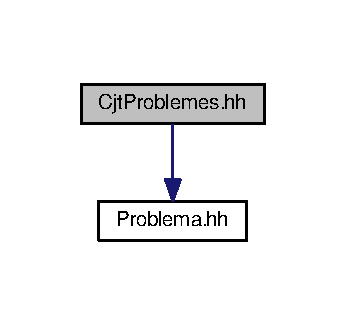
\includegraphics[width=166pt]{_cjt_problemes_8hh__incl}
\end{center}
\end{figure}
\subsection*{Clases}
\begin{DoxyCompactItemize}
\item 
class \mbox{\hyperlink{class_cjt_problemes}{Cjt\+Problemes}}
\begin{DoxyCompactList}\small\item\em Representa un conjunt de problemes. \end{DoxyCompactList}\end{DoxyCompactItemize}


\subsection{Descripción detallada}
Especificació de la clase \mbox{\hyperlink{class_cjt_problemes}{Cjt\+Problemes}}. 


\hypertarget{_cjt_sessions_8hh}{}\doxysection{Referencia del Archivo Cjt\+Sessions.\+hh}
\label{_cjt_sessions_8hh}\index{CjtSessions.hh@{CjtSessions.hh}}


Especificació de la classe \mbox{\hyperlink{class_cjt_sessions}{Cjt\+Sessions}}.  


Dependencia gráfica adjunta para Cjt\+Sessions.\+hh\+:
% FIG 0
\doxysubsection*{Clases}
\begin{DoxyCompactItemize}
\item 
class \mbox{\hyperlink{class_cjt_sessions}{Cjt\+Sessions}}
\begin{DoxyCompactList}\small\item\em Representa un Conjunt de sessions (\mbox{\hyperlink{class_sessio}{Sessio}}). \end{DoxyCompactList}\end{DoxyCompactItemize}


\doxysubsection{Descripción detallada}
Especificació de la classe \mbox{\hyperlink{class_cjt_sessions}{Cjt\+Sessions}}. 


\hypertarget{_cjt_usuaris_8hh}{}\section{Referencia del Archivo Cjt\+Usuaris.\+hh}
\label{_cjt_usuaris_8hh}\index{Cjt\+Usuaris.\+hh@{Cjt\+Usuaris.\+hh}}


Especificació de la classe \mbox{\hyperlink{class_cjt_usuaris}{Cjt\+Usuaris}}.  


Dependencia gráfica adjunta para Cjt\+Usuaris.\+hh\+:
\nopagebreak
\begin{figure}[H]
\begin{center}
\leavevmode
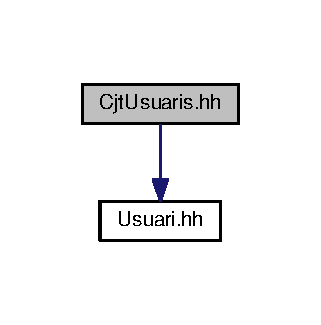
\includegraphics[width=154pt]{_cjt_usuaris_8hh__incl}
\end{center}
\end{figure}
\subsection*{Clases}
\begin{DoxyCompactItemize}
\item 
class \mbox{\hyperlink{class_cjt_usuaris}{Cjt\+Usuaris}}
\begin{DoxyCompactList}\small\item\em Representa el conjunt de tots els usuaris\end{DoxyCompactList}\end{DoxyCompactItemize}


\subsection{Descripción detallada}
Especificació de la classe \mbox{\hyperlink{class_cjt_usuaris}{Cjt\+Usuaris}}. 


\hypertarget{_curs_8hh}{}\section{Referencia del Archivo Curs.\+hh}
\label{_curs_8hh}\index{Curs.\+hh@{Curs.\+hh}}


Especificació de la clase \mbox{\hyperlink{class_curs}{Curs}}.  


Dependencia gráfica adjunta para Curs.\+hh\+:\nopagebreak
\begin{figure}[H]
\begin{center}
\leavevmode
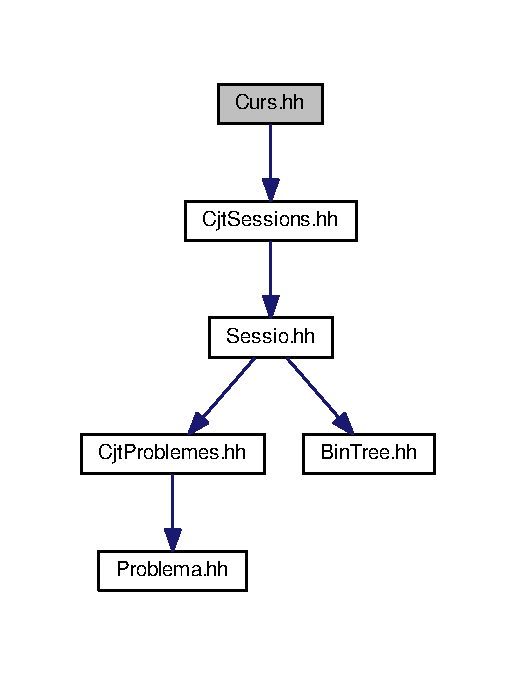
\includegraphics[width=248pt]{_curs_8hh__incl}
\end{center}
\end{figure}
\subsection*{Clases}
\begin{DoxyCompactItemize}
\item 
class \mbox{\hyperlink{class_curs}{Curs}}
\begin{DoxyCompactList}\small\item\em Representa un \mbox{\hyperlink{class_curs}{Curs}}. \end{DoxyCompactList}\end{DoxyCompactItemize}


\subsection{Descripción detallada}
Especificació de la clase \mbox{\hyperlink{class_curs}{Curs}}. 


\hypertarget{main_8cc}{}\section{Referencia del Archivo main.\+cc}
\label{main_8cc}\index{main.\+cc@{main.\+cc}}


Programa principal.  


Dependencia gráfica adjunta para main.\+cc\+:\nopagebreak
\begin{figure}[H]
\begin{center}
\leavevmode
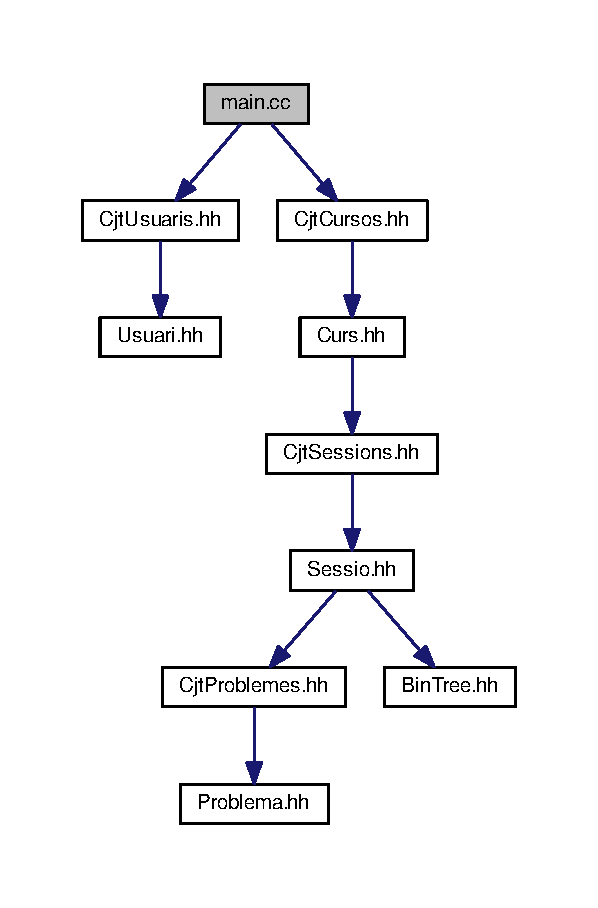
\includegraphics[width=287pt]{main_8cc__incl}
\end{center}
\end{figure}
\subsection*{Funciones}
\begin{DoxyCompactItemize}
\item 
int \mbox{\hyperlink{main_8cc_ae66f6b31b5ad750f1fe042a706a4e3d4}{main}} ()
\end{DoxyCompactItemize}


\subsection{Descripción detallada}
Programa principal. 



\subsection{Documentación de las funciones}
\mbox{\Hypertarget{main_8cc_ae66f6b31b5ad750f1fe042a706a4e3d4}\label{main_8cc_ae66f6b31b5ad750f1fe042a706a4e3d4}} 
\index{main.\+cc@{main.\+cc}!main@{main}}
\index{main@{main}!main.\+cc@{main.\+cc}}
\subsubsection{\texorpdfstring{main()}{main()}}
{\footnotesize\ttfamily int main (\begin{DoxyParamCaption}{ }\end{DoxyParamCaption})}



Definición en la línea 8 del archivo main.\+cc.


\begin{DoxyCode}
8            \{
9     \mbox{\hyperlink{class_cjt_problemes}{CjtProblemes}} cjtProb;
10     \mbox{\hyperlink{class_cjt_sessions}{CjtSessions}} cjtSes;
11     \mbox{\hyperlink{class_cjt_cursos}{CjtCursos}} cjtCurs;
12     \mbox{\hyperlink{class_cjt_usuaris}{CjtUsuaris}} cjtUs;
13 
14     \textcolor{keywordtype}{string} op;
15 
16     cjtProb.\mbox{\hyperlink{class_cjt_problemes_ac320f52e566402ed341d2f67176be14a}{llegir\_problemes\_inicials}}();
17     cjtSes.\mbox{\hyperlink{class_cjt_sessions_a4ea0fafab13c9db8fe385f62fb572fc0}{llegir\_sessions\_inicials}}();
18     cjtCurs.\mbox{\hyperlink{class_cjt_cursos_a970aa3d7caa26ed983ccd71e4bfd0adf}{llegir\_cursos\_inicials}}();
19     cjtUs.\mbox{\hyperlink{class_cjt_usuaris_acb8d525b500b034d277c48197d16a682}{llegir\_usuaris\_inicials}}();
20 
21     cin >> op;
22     \textcolor{keywordflow}{while}(op != \textcolor{stringliteral}{"fin"}) \{
23         \textcolor{keywordtype}{string} auxString;
24         \textcolor{keywordtype}{int} auxInt;
25         \textcolor{keywordflow}{if} (op == \textcolor{stringliteral}{"np"} or op == \textcolor{stringliteral}{"nuevo\_problema"}) \{
26             cin >> auxString;
27             
28             \textcolor{keywordflow}{if}(not cjtProb.\mbox{\hyperlink{class_cjt_problemes_a27f5be292f79fd47915093fb84013e67}{existeix\_problema}}(auxString))\{
29                 cjtProb.\mbox{\hyperlink{class_cjt_problemes_a7a41c837128c629f7a4dcf81b1592581}{nou\_problema}}(auxString);
30             \}
31             \textcolor{keywordflow}{else} cout<<\textcolor{stringliteral}{"ERROR, ja existeix el problema"}<<endl;
32         \}
33 
34         \textcolor{keywordflow}{else} \textcolor{keywordflow}{if} (op == \textcolor{stringliteral}{"ns"} or op == \textcolor{stringliteral}{" nueva\_sesion "}) \{
35             cin >> auxString;
36 
37             \textcolor{keywordflow}{if}(not cjtSes.\mbox{\hyperlink{class_cjt_sessions_ae0d6dfe6e1bab2746fa03dc852f2f4a9}{existeix\_sessio}}(auxString))\{
38                 cjtSes.\mbox{\hyperlink{class_cjt_sessions_ac6e00a3727d5ece89965a4f38d707273}{nova\_sessio}}( auxString );
39             \}
40             \textcolor{keywordflow}{else} cout<<\textcolor{stringliteral}{"ERROR, ja existeix la Sessió"}<<endl;
41         \}
42         \textcolor{keywordflow}{else} \textcolor{keywordflow}{if} (op == \textcolor{stringliteral}{"nc"} or op == \textcolor{stringliteral}{" nuevo\_curso "}) \{
43             cjtCurs.\mbox{\hyperlink{class_cjt_cursos_a3d4778b4572a99e1109d6376f439255e}{nou\_curs}}();
44         \}
45         \textcolor{keywordflow}{else} \textcolor{keywordflow}{if} (op == \textcolor{stringliteral}{"a"} or op == \textcolor{stringliteral}{" alta\_usuario "}) \{
46             cin >> auxString;
47 
48             \textcolor{keywordflow}{if} (cjtUs.\mbox{\hyperlink{class_cjt_usuaris_a0d3f318f95ecfdae0f7420113cc73ab0}{existeix\_usuari}}( auxString )) \{
49                 \mbox{\hyperlink{class_usuari}{Usuari}} u = \mbox{\hyperlink{class_usuari}{Usuari}}(auxString);
50                 cjtUs.\mbox{\hyperlink{class_cjt_usuaris_a40b8eb64e9dc22e3cf0ee38d52d48e20}{alta\_usuari}}(u);
51             \}
52             \textcolor{keywordflow}{else} cout << \textcolor{stringliteral}{"ERROR: no existeix el Curs"}<< auxInt << endl;
53         \}
54 
55         \textcolor{keywordflow}{else} \textcolor{keywordflow}{if} (op == \textcolor{stringliteral}{"b"} or op == \textcolor{stringliteral}{" baja\_usuario "}) \{
56             cin >> auxString;
57 
58              \textcolor{keywordflow}{if} (cjtUs.\mbox{\hyperlink{class_cjt_usuaris_a0d3f318f95ecfdae0f7420113cc73ab0}{existeix\_usuari}}( auxString )) \{
59                 cjtUs.\mbox{\hyperlink{class_cjt_usuaris_a8aa977e92fd28d1c1dd1604ec3ed21e8}{baixa\_usuari}}( auxString );
60             \}
61             \textcolor{keywordflow}{else} cout << \textcolor{stringliteral}{"ERROR: no existeix el Curs"}<< auxInt << endl;
62         \}
63 
64         \textcolor{keywordflow}{else} \textcolor{keywordflow}{if} (op == \textcolor{stringliteral}{"i"} or op == \textcolor{stringliteral}{" inscribir\_curso "}) \{
65             cin >> auxString >> auxInt;
66 
67             \textcolor{keywordflow}{if} (cjtUs.\mbox{\hyperlink{class_cjt_usuaris_a0d3f318f95ecfdae0f7420113cc73ab0}{existeix\_usuari}}(auxString) and cjtCurs.
      \mbox{\hyperlink{class_cjt_cursos_ad12b1174de2a5f09cb0c2558645d74dc}{existeix\_curs}}(auxInt)) \{
68                 \mbox{\hyperlink{class_usuari}{Usuari}} user = cjtUs.\mbox{\hyperlink{class_cjt_usuaris_a01e702bce964b2a96af36fcd9a820b74}{accedir\_usuari}}( auxString );
69                 \textcolor{keywordflow}{if} (user.\mbox{\hyperlink{class_usuari_a0d20c2d77d8231d9a7e3e00a42a7e7c8}{esta\_inscrit}}() == 0) user.\mbox{\hyperlink{class_usuari_af7f2d183e02eec8428bf48df89efb763}{inscribir\_curso}}( auxInt );
70                 \textcolor{keywordflow}{else} cout << \textcolor{stringliteral}{"ERROR: l'Usuari ja està inscrit a un curs."} << endl;
71 
72             \}
73             \textcolor{keywordflow}{else} cout << \textcolor{stringliteral}{"ERROR: L'Usuari o el curs no existeixen."} << endl;
74         \}
75 
76         \textcolor{keywordflow}{else} \textcolor{keywordflow}{if} (op == \textcolor{stringliteral}{"cu"} or op == \textcolor{stringliteral}{" curso\_usuario "}) \{
77             cin >> auxString;
78 
79              \textcolor{keywordflow}{if} (cjtUs.\mbox{\hyperlink{class_cjt_usuaris_a0d3f318f95ecfdae0f7420113cc73ab0}{existeix\_usuari}}( auxString )) \{
80                 \mbox{\hyperlink{class_usuari}{Usuari}} user = cjtUs.\mbox{\hyperlink{class_cjt_usuaris_a01e702bce964b2a96af36fcd9a820b74}{accedir\_usuari}} ( auxString );
81                 cout << user.\mbox{\hyperlink{class_usuari_a0d20c2d77d8231d9a7e3e00a42a7e7c8}{esta\_inscrit}}() <<endl;
82             \}
83             \textcolor{keywordflow}{else} cout << \textcolor{stringliteral}{"ERROR: no existeix el Curs"}<< auxInt << endl;
84         \}
85 
86         \textcolor{keywordflow}{else} \textcolor{keywordflow}{if} (op == \textcolor{stringliteral}{"sp"} or op == \textcolor{stringliteral}{" sesion\_problema "}) \{
87             cin >> auxInt >> auxString;
88             \textcolor{keywordflow}{if} (not cjtCurs.\mbox{\hyperlink{class_cjt_cursos_ad12b1174de2a5f09cb0c2558645d74dc}{existeix\_curs}}( auxInt)) cout << \textcolor{stringliteral}{"ERROR: no existeix el Curs"} << 
      auxInt << endl;
89             \textcolor{keywordflow}{else} \textcolor{keywordflow}{if} (not cjtProb.\mbox{\hyperlink{class_cjt_problemes_a27f5be292f79fd47915093fb84013e67}{existeix\_problema}}( auxString)) cout << \textcolor{stringliteral}{"ERROR: no
       existeix el Problema"} << auxString << endl;
90             \textcolor{keywordflow}{else} \{
91                 \mbox{\hyperlink{class_curs}{Curs}} curs = cjtCurs.\mbox{\hyperlink{class_cjt_cursos_aaff9556e6d0f2b55e74fb757ffd51e42}{accedir\_curs}}( auxInt );
92                 cout << curs.\mbox{\hyperlink{class_curs_ab9c0e100a9c7231c5c96911c94602fff}{trobar\_sessio}}( auxString ) << endl;
93             \}
94         \}
95 
96         \textcolor{keywordflow}{else} \textcolor{keywordflow}{if} (op == \textcolor{stringliteral}{"pr"} or op == \textcolor{stringliteral}{" problemas\_resueltos "}) \{
97             cin >> auxString;
98             \textcolor{keywordflow}{if}(cjtUs.\mbox{\hyperlink{class_cjt_usuaris_a0d3f318f95ecfdae0f7420113cc73ab0}{existeix\_usuari}}( auxString)) \{
99                 \mbox{\hyperlink{class_usuari}{Usuari}} user = cjtUs.\mbox{\hyperlink{class_cjt_usuaris_a01e702bce964b2a96af36fcd9a820b74}{accedir\_usuari}}( auxString );
100                 user.\mbox{\hyperlink{class_usuari_a3ef9f5ec04fe13ecfaf6d2f02bcd30bd}{problemes\_resolts}}();
101             \}
102             \textcolor{keywordflow}{else} cout << \textcolor{stringliteral}{"ERROR: no existeix l'Usuari"} << auxString << endl;
103         \}
104         \textcolor{keywordflow}{else} \textcolor{keywordflow}{if} (op == \textcolor{stringliteral}{"pe"} or op == \textcolor{stringliteral}{" problemas\_enviables "}) \{
105             cin >> auxString;
106             \textcolor{keywordflow}{if}(cjtUs.\mbox{\hyperlink{class_cjt_usuaris_a0d3f318f95ecfdae0f7420113cc73ab0}{existeix\_usuari}}( auxString)) \{
107                 \mbox{\hyperlink{class_usuari}{Usuari}} user = cjtUs.\mbox{\hyperlink{class_cjt_usuaris_a01e702bce964b2a96af36fcd9a820b74}{accedir\_usuari}}( auxString );
108                 user.\mbox{\hyperlink{class_usuari_a84e0532f6b7ae4c4022e4739ca7abade}{problemes\_enviables}}();
109             \}
110             \textcolor{keywordflow}{else} cout << \textcolor{stringliteral}{"ERROR: no existeix l'Usuari"} << auxString << endl;
111         \}
112 
113         \textcolor{keywordflow}{else} \textcolor{keywordflow}{if} (op == \textcolor{stringliteral}{"e"} or op == \textcolor{stringliteral}{" envio "}) \{
114             \textcolor{keywordtype}{bool} r;
115             \textcolor{keywordtype}{string} p;
116             cin >> auxString >> p >> r;
117 
118             \mbox{\hyperlink{class_usuari}{Usuari}} user = cjtUs.\mbox{\hyperlink{class_cjt_usuaris_a01e702bce964b2a96af36fcd9a820b74}{accedir\_usuari}}( auxString );
119             \mbox{\hyperlink{class_problema}{Problema}} prob = cjtProb.\mbox{\hyperlink{class_cjt_problemes_ae0db90032709a9d6af8312b93877d514}{accedir\_problema}}( p );
120 
121             prob.\mbox{\hyperlink{class_problema_a769d7920810acf042cdd6aa9c3236a0c}{actualitzar\_stats}}( r );
122             user.\mbox{\hyperlink{class_usuari_ab47d77ad6eb5d9139f464c226fca2af4}{actualitzar\_stats}}(auxInt, r);
123 
124             \textcolor{keywordflow}{if} ( r ) \{
125                 user.\mbox{\hyperlink{class_usuari_a3cb6bb4ab49c3f858f3588c77af11527}{curs\_completat}}();
126             \}
127         \}
128 
129         \textcolor{keywordflow}{else} \textcolor{keywordflow}{if} (op == \textcolor{stringliteral}{"lp"} or op == \textcolor{stringliteral}{" listar\_problemas "}) \{
130             cjtProb.\mbox{\hyperlink{class_cjt_problemes_a976ab13903046970b2e128a3fa4df8fa}{llistat\_problemes}}();
131         \}
132 
133         \textcolor{keywordflow}{else} \textcolor{keywordflow}{if} (op == \textcolor{stringliteral}{"ep"} or op == \textcolor{stringliteral}{" escribir\_problema "}) \{
134             cin >> auxString;
135             \textcolor{keywordflow}{if} (cjtProb.\mbox{\hyperlink{class_cjt_problemes_a27f5be292f79fd47915093fb84013e67}{existeix\_problema}}( auxString )) \{
136                 \mbox{\hyperlink{class_problema}{Problema}} prob = cjtProb.\mbox{\hyperlink{class_cjt_problemes_ae0db90032709a9d6af8312b93877d514}{accedir\_problema}} ( auxString );
137                 prob.\mbox{\hyperlink{class_problema_a6faae2ee8a1812951b22565cc234e8a4}{escriure\_problema}}();
138             \}
139             \textcolor{keywordflow}{else} cout << \textcolor{stringliteral}{"ERROR: no existeix el Problema"} << auxString << endl;
140         \}
141 
142         \textcolor{keywordflow}{else} \textcolor{keywordflow}{if} (op == \textcolor{stringliteral}{"ls"} or op == \textcolor{stringliteral}{" listar\_sesiones "}) \{
143             cjtSes.\mbox{\hyperlink{class_cjt_sessions_a1e4f04be3e5da3d8f9091620d56ea355}{llistat\_sessions}}();
144         \}
145 
146         \textcolor{keywordflow}{else} \textcolor{keywordflow}{if} (op == \textcolor{stringliteral}{"es"} or op == \textcolor{stringliteral}{" escribir\_sesion "}) \{
147             cin >> auxString;
148 
149             \textcolor{keywordflow}{if} (cjtSes.\mbox{\hyperlink{class_cjt_sessions_ae0d6dfe6e1bab2746fa03dc852f2f4a9}{existeix\_sessio}}( auxString )) \{
150                 \mbox{\hyperlink{class_sessio}{Sessio}} ses = cjtSes.\mbox{\hyperlink{class_cjt_sessions_a373d89dde7bb62322feb50f3a299d5de}{accedir\_sessio}} ( auxString );
151                 ses.\mbox{\hyperlink{class_sessio_a3d0efb2a3395d34c04369e15bf29824f}{escriure\_sessio}}();
152             \}
153             \textcolor{keywordflow}{else} cout << \textcolor{stringliteral}{"ERROR: no existeix la Sessió"} << auxString << endl;
154 
155         \}
156 
157         \textcolor{keywordflow}{else} \textcolor{keywordflow}{if} (op == \textcolor{stringliteral}{"lc"} or op == \textcolor{stringliteral}{" listar\_cursos "}) \{
158             cjtCurs.\mbox{\hyperlink{class_cjt_cursos_a9a772bfad772e507fa9b8f5194b13873}{llistat\_cursos}}();
159         \}
160 
161         \textcolor{keywordflow}{else} \textcolor{keywordflow}{if} (op == \textcolor{stringliteral}{"ec"} or op == \textcolor{stringliteral}{" escribir\_curso "}) \{
162             cin >> auxInt;
163 
164              \textcolor{keywordflow}{if} (cjtCurs.\mbox{\hyperlink{class_cjt_cursos_ad12b1174de2a5f09cb0c2558645d74dc}{existeix\_curs}}( auxInt )) \{
165                 \mbox{\hyperlink{class_curs}{Curs}} curs = cjtCurs.\mbox{\hyperlink{class_cjt_cursos_aaff9556e6d0f2b55e74fb757ffd51e42}{accedir\_curs}} ( auxInt );
166                 curs.\mbox{\hyperlink{class_curs_a54b500f472e5ae51395bca6fe1e0bd09}{escriure\_curs}}();
167             \}
168             \textcolor{keywordflow}{else} cout << \textcolor{stringliteral}{"ERROR: no existeix el Curs"}<< auxInt << endl;
169 
170         \}
171 
172         \textcolor{keywordflow}{else} \textcolor{keywordflow}{if} (op == \textcolor{stringliteral}{"lu"} or op == \textcolor{stringliteral}{" listar\_usuarios "}) \{
173             cjtUs.\mbox{\hyperlink{class_cjt_usuaris_a28020e6e834b3c483198285fb35436fc}{llistat\_usuaris}}();
174         \}
175 
176         \textcolor{keywordflow}{else} \textcolor{keywordflow}{if} (op == \textcolor{stringliteral}{"eu"} or op == \textcolor{stringliteral}{" escribir\_usuario "}) \{
177             cin >> auxString;
178 
179              \textcolor{keywordflow}{if} (cjtUs.\mbox{\hyperlink{class_cjt_usuaris_a0d3f318f95ecfdae0f7420113cc73ab0}{existeix\_usuari}}( auxString )) \{
180                 \mbox{\hyperlink{class_usuari}{Usuari}} user = cjtUs.\mbox{\hyperlink{class_cjt_usuaris_a01e702bce964b2a96af36fcd9a820b74}{accedir\_usuari}} ( auxString );
181                 user.\mbox{\hyperlink{class_usuari_a19ce3acaf6693208eed30686bd79c30e}{escriure\_usuari}}();
182             \}
183             \textcolor{keywordflow}{else} cout << \textcolor{stringliteral}{"ERROR: no existeix el Curs"}<< auxInt << endl;
184         \}
185 
186         cin >> op;
187     \}
188 \}
\end{DoxyCode}

\hypertarget{_problema_8hh}{}\section{Referencia del Archivo Problema.\+hh}
\label{_problema_8hh}\index{Problema.\+hh@{Problema.\+hh}}


Especificació de la classe \mbox{\hyperlink{class_problema}{Problema}}.  


\subsection*{Clases}
\begin{DoxyCompactItemize}
\item 
class \mbox{\hyperlink{class_problema}{Problema}}
\begin{DoxyCompactList}\small\item\em Representa un \mbox{\hyperlink{class_problema}{Problema}}. \end{DoxyCompactList}\end{DoxyCompactItemize}


\subsection{Descripción detallada}
Especificació de la classe \mbox{\hyperlink{class_problema}{Problema}}. 


\hypertarget{_sessio_8hh}{}\doxysection{Referencia del Archivo Sessio.\+hh}
\label{_sessio_8hh}\index{Sessio.hh@{Sessio.hh}}


Especificació de la classe \mbox{\hyperlink{class_sessio}{Sessio}}.  


Dependencia gráfica adjunta para Sessio.\+hh\+:
% FIG 0
\doxysubsection*{Clases}
\begin{DoxyCompactItemize}
\item 
class \mbox{\hyperlink{class_sessio}{Sessio}}
\begin{DoxyCompactList}\small\item\em Representa una \mbox{\hyperlink{class_sessio}{Sessio}}. \end{DoxyCompactList}\end{DoxyCompactItemize}


\doxysubsection{Descripción detallada}
Especificació de la classe \mbox{\hyperlink{class_sessio}{Sessio}}. 


\hypertarget{_usuari_8hh}{}\section{Referencia del Archivo Usuari.\+hh}
\label{_usuari_8hh}\index{Usuari.\+hh@{Usuari.\+hh}}


Especificació de la classe \mbox{\hyperlink{class_usuari}{Usuari}}.  


\subsection*{Clases}
\begin{DoxyCompactItemize}
\item 
class \mbox{\hyperlink{class_usuari}{Usuari}}
\begin{DoxyCompactList}\small\item\em Representa un \mbox{\hyperlink{class_usuari}{Usuari}}. \end{DoxyCompactList}\end{DoxyCompactItemize}


\subsection{Descripción detallada}
Especificació de la classe \mbox{\hyperlink{class_usuari}{Usuari}}. 


%--- End generated contents ---

% Index
\backmatter
\newpage
\phantomsection
\clearemptydoublepage
\addcontentsline{toc}{chapter}{Índice}
\printindex

\end{document}
